% Do not compile this file directly, but instead the thesis_a4 or the thesis_elec one.

% For encoding
\usepackage[T1]{fontenc}
\usepackage[utf8]{inputenc}
\usepackage[english]{babel}

% For quotes
\usepackage{epigraph}

% Additional math symbols 
\usepackage{amssymb}

% Biblatex provides much more flexibility than bibtex for bibliography and citation management
% For quotes used by biblatex
\usepackage{csquotes}
% alphabetic style for labeled citations, maxbibnames to 99 to avoid "et al." in bibliography, giveninits to true to keep only given name initials
\usepackage[style=alphabetic,maxbibnames=99,giveninits=true]{biblatex}
% Add your bib files here
\addbibresource{biblio.bib}

% When calling "\fullcite", prevent it from "et al."ing
\preto\fullcite{\AtNextCite{\defcounter{maxnames}{99}}}
% Some bib fields might be useless to show, the following lines configure this
\AtEveryBibitem{% Clean up the bibtex rather than editing it
	\clearlist{language}
	\ifentrytype{online}{}{% Remove url except for @online
		\clearfield{url}
		\clearfield{urldate}
	}
}

% The following commands allow citing own contributions in the "Bibliographic notes" section without appearing in the "References" one
\DeclareBibliographyCategory{fullcited}
\newcommand{\mybibexclude}[1]{\addtocategory{fullcited}{#1}}
% The "\myfullcite" command to be used in the "Bibliographic notes" section
\newcommand{\myfullcite}[1]{\fullcite{#1}.\mybibexclude{#1}}
%\usepackage{cite}
%\usepackage{bibentry}

% Linux Libertine is a nice font; notice that we scale the "\texttt", as the default tt font is too large
\usepackage[ttscale=.875]{libertine}
% Also adapt the math mode
\usepackage[libertine]{newtxmath}

% Enable to customize the format of the "\today" command
\usepackage{datetime}

% Add key-value interface for "\includegraphics" command
\usepackage{graphicx}

% Provide "\multirow" for tabular environment
\usepackage{multirow}

% Enable URL command with hyperlinks, while forcing correct line-breaks (see https://tex.stackexchange.com/a/3034)
% Also disable the neon boxes around hyperlinks (https://tex.stackexchange.com/a/12408)
\PassOptionsToPackage{hyphens}{url}\usepackage[hidelinks]{hyperref}

% Provide additional features to the verbatim environment
\usepackage{moreverb}

% Enable figure and table (sub)captioning, and configure their font
\usepackage[font=small]{caption}
\captionsetup[figure]{labelfont=bf,textfont=bf}
\captionsetup[table]{labelfont=bf,textfont=bf}
\usepackage{subcaption}

% Extend the interface of floating objects like figures and tables
\usepackage{float}

% Provide framed and coloured boxes
\usepackage{mdframed}

% Flexible handling of verbatim environment
\usepackage{fancyvrb}

% Macro package to create graphics, with its "user-friendly" syntax Tikz
\usepackage{pgf}
\usepackage{tikz}
% Enable drawing plots by directly specifying them in Tex
\usepackage{pgfplots}
% This is just loading optimizations
\usetikzlibrary{shapes.misc,shapes,external,pgfplots.statistics}
\usepgfplotslibrary{groupplots}

% Provide facilities to insert (or not) spaces after macros (with "\xspace")
\usepackage{xspace}

% Provide the text companion font
\usepackage{textcomp}

% For figures in network protocol specifications
\usepackage{bytefield}

% For LuaTex, provide utility commands built-in in pdflatex
\usepackage{pdftexcmds}

% Provide support to rotate figures
\usepackage{rotating}

% To include PDF documents inside the current one
\usepackage{pdfpages}

% Allow wrapping text around figures
\usepackage{wrapfig}

% Define colors
\usepackage{xcolor}

% Enable algorithm definition
\usepackage{amsmath}
\usepackage{algorithm}
\usepackage[noend]{algpseudocode}

\renewcommand{\algorithmicrequire}{\textbf{Input:}}
\renewcommand{\algorithmicensure}{\textbf{Output:}}

% Change the section numbering depth to 3 levels
\setcounter{secnumdepth}{3}
% Idem for the table of contents
\setcounter{tocdepth}{3}

% Replace the item bullets by a nice gray square
\renewcommand{\labelitemi}{\color{gray} \scriptsize$\blacksquare$}

% Placing TODOs in Latex
\usepackage{todonotes}
% Proposed options: inline TODOs instead of margin ones, disable TODOs
%\presetkeys{todonotes}{inline,linecolor=red,backgroundcolor=red!25,disable}{}

% I hope you won't require this package once your thesis is completed :-)
\usepackage{lipsum}

% To tune the chapter format
\usepackage{pbox}
\usepackage[clearempty,newlinetospace,raggedright,small,explicit]{titlesec}

% For the chapterformatting
\definecolor{gray65}{gray}{0.65}

\newcommand{\size}[2]{{\fontsize{#1}{0}\selectfont #2}}
\newcommand{\sizeline}[3]{{\fontsize{#1}{#2}\selectfont #3}}
\newenvironment{sizepar}[2]
{\par\fontsize{#1}{#2}\selectfont}
{\par}

\newcommand{\printchapternumber}{%
	\begingroup\renewcommand{\arraystretch}{0}%
	\begin{tabular}{@{}c@{}}\size{56}{\thechapter}\end{tabular}%
	\endgroup
}

\titleformat{\chapter}[block]
{\bfseries\filright}
{}
{0pt}
{%
	\parbox{.865\textwidth}{\raggedright\Huge\selectfont#1}%
	\hspace{6pt}%
	\color{gray65}\vrule width 1.5pt
	\hspace{6pt}%
	\printchapternumber
}

\titleformat{name=\chapter,numberless}[block]
{\bfseries\filright}
{}
{0pt}
{%
	\parbox{\textwidth}{\raggedright\Huge\selectfont#1}%
}

\titlespacing*{\chapter}{0pt}{0pt}{60pt}

%%%
% Short date format : May 2019
\newdateformat{monthyeardate}{\monthname[\THEMONTH] \THEYEAR}

%%%% Short commands %%%
% Title of the thesis
\newcommand{\thesisTitle}{A Wonderful Title for Your Thesis}

% Your name here (and keep the "\xspace"!)
\newcommand{\thesisAuthor}{Jean-Luc Picard\xspace}

% Clear an empty double page
\newcommand{\clearemptydoublepage}{%
	\newpage{\pagestyle{empty}\cleardoublepage}}

% Define here all your user-defined commands here
\newcommand{\ie}{\textit{i.e.}}
\newcommand{\eg}{\textit{e.g.}}
\newcommand{\ed}[1]{\textsf{\textbf{[#1]}}}


%\newcommand{\rtt}{\textsf{\small{RTT}}}
%\newcommand{\tcp}{{\textsf{\tiny{TCP}}}}
\newcommand{\ip}{{\textsc IP}\xspace}
\newcommand{\tcp}{{\textsc TCP}\xspace}
\newcommand{\mptcp}{Multi\-path \tcp}
\newcommand{\wifi}{{Wi-Fi}\xspace}
\newcommand{\socks}{{\textsc SOCKS}\xspace}
\newcommand{\http}{{\textsc HTTP}\xspace}
\newcommand{\get}{{\textsc GET}\xspace}

\newcommand{\quic}{{\textsc QUIC}\xspace}

\newcommand{\textbio}[1]{{\biolinum{\textit{#1}}}\xspace}
\newcommand{\textbiob}[1]{{\biolinum{\textbf{#1}}}\xspace}
\newcommand{\textbion}[1]{{\biolinum{#1}}\xspace}

\newcommand{\fullmesh}{{\texttt{full-mesh}}\xspace}

\newcommand{\default}{{\texttt{default}}\xspace}
\newcommand{\redundant}{{\texttt{redundant}}\xspace}

\newcommand{\multipathtester}{{\sc{MultipathTester}}\xspace}
\newcommand{\ipv}[1]{{\textsc IPv{#1}}\xspace}

\newcommand{\nobk}{{\sc{No Backup}}\xspace}
\newcommand{\bk}{{\sc{Backup}}\xspace}
\newcommand{\ietfbk}{{\sc{IETF Backup}}\xspace}
\newcommand{\multimob}{{\sc{MultiMob}}\xspace}

\newcommand{\mpquicimpl}{{\textsc mp-quic}\xspace}

\newcommand{\syn}{{\sc Syn}\xspace}
\newcommand{\ack}{{\sc Ack}\xspace}
\newcommand{\rst}{{\sc Rst}\xspace}
%\newcommand{\dataack}{{\sc Data Ack}\xspace}
\newcommand{\datafin}{{\sc Data Fin}\xspace}
\newcommand{\fin}{{\sc Fin}\xspace}
\newcommand{\mpcapable}{{\sc Mp Capable}\xspace}
\newcommand{\mpjoin}{{\sc Mp Join}\xspace}
\newcommand{\fastjoinin}{{\sc Fast Join In}\xspace}
\newcommand{\fastjoinout}{{\sc Fast Join Out}\xspace}
\newcommand{\addaddr}{{\sc Add Addr}\xspace}
\newcommand{\removeaddr}{{\sc Remove Addr}\xspace}
\newcommand{\fastclose}{{\sc Fast Close}\xspace}


\begin{document}
\thispagestyle{empty}

\begin{center}
\vspace{0.5cm}
% The title is small capped, I found it nice to have but not required
{\bf \huge \textsc \thesisTitle}\\
~\\
\vspace{0.5cm}
\large \thesisAuthor\\
\vspace{1cm}
{\em Thesis submitted in partial fulfillment of the requirements for\\
the Degree of Doctor in Applied Sciences}\\
\vspace{1cm}
\monthyeardate\today\\
\vspace{1cm}
ICTEAM\\
Louvain School of Engineering\\
Universit\'{e} catholique de Louvain\\
Louvain-la-Neuve\\
Belgium\\
\end{center}

\vspace{6.5cm}

\noindent\underline{\bf Thesis Committee:}\\
\begin{tabular}{lr}
Pr.~Wonderful {\bf Supervisor} (Advisor) & UCLouvain/ICTEAM, Belgium\\
Pr.~Good {\bf Doctor} & UCLouvain/ICTEAM, Belgium\\
Pr.~Another {\bf Guy} & Another University, World\\
\end{tabular}
\newpage
\thispagestyle{empty}

\noindent
{\Large \thesisTitle}\\
\vspace{0.5cm}
by \thesisAuthor\\
\vspace{1.5cm}

\noindent
$\copyright$ \thesisAuthor 2019\\
ICTEAM\\
Universit\'e catholique de Louvain\\
Place Sainte-Barbe, 2\\
1348 Louvain-la-Neuve\\
Belgium

\vspace{10cm}

\noindent
This work was partially supported by the F.R.S-FNRS.

% This one is optional
\newpage

\thispagestyle{empty}
\null\vfill

%\newlength\longest
%\settowidth\longest{\huge\itshape tell you a TCP joke...}
\parbox{\textwidth}{%
	\raggedleft{\huge\itshape%
		Hey, I want to \\ 
		tell you a TCP joke... \\
	}   
	\raggedleft\Large\MakeUppercase{Anonymous}\par%
}

\vfill\vfill

\clearemptydoublepage
% Start counting with latin numbers
\frontmatter
\clearemptydoublepage

\addcontentsline{toc}{chapter}{Preamble}
\chapter*{Preamble}
\markboth{Preamble}{Preamble}

We will put here some text that will motivate the need of your thesis.
Because the world needs your input, you feel invested in a four-year long quest to fill in the gap between your dreams and the reality.
In particular, the following explains why the world is wrong.

\lipsum[42]

This thesis bridges this gap to achieve very interesting results.
In particular, the main contributions of this thesis are the following.

\begin{itemize}
\item \textit{A first very interesting contribution to highlight.} \\

We here describe some lines to show what you first made.
\lipsum[2]

\item \textit{A second element based on your first contribution.} \\

\lipsum[5-6]

\item \textit{Now forget the first two contributions to see this one.} \\

\lipsum[9]

\item \textit{A last point to close the loop.} \\

\lipsum[13] 

\end{itemize}

The thesis is organized as follows.
Chapter~\ref{sec:tips} provides some useful examples for the thesis.
Then, Chapter~\ref{sec:long} illustrates how a long text looks like.
Finally, Chapter~\ref{sec:ccl} concludes this template.

\newpage

\section*{Bibliographic notes}

\subsection*{Conference Publications}

\begin{enumerate}

\item \myfullcite{picard_first_2017}
\item \myfullcite{picard_unhoped_2018}

\end{enumerate}

\subsection*{Posters and Demos}

\begin{enumerate}
\item \myfullcite{legolas_bow_2018}

\end{enumerate}

\subsection*{Journal Publications}

\begin{enumerate}
\item \myfullcite{picard_voyager_2017}
\item \myfullcite{wayne_improving_2019}

\end{enumerate}

\subsection*{Miscellaneous Contributions}

\begin{enumerate}
\item \myfullcite{picard_pandora_2019}
\end{enumerate}

\clearemptydoublepage

\addcontentsline{toc}{chapter}{Acknowledgments}
\chapter*{Acknowledgments}
\markboth{Acknowledgments}{Acknowledgments}

While this version was first brought by Quentin De Coninck, it relies on the templates of numerous previous Ph.D. students, including David Lebrun, Olivier Tilmans and Fabien Duchêne.
\clearemptydoublepage

\addcontentsline{toc}{chapter}{Table of Contents}
\tableofcontents
\clearemptydoublepage

% Start the actual count
\mainmatter

\chapter{Some Examples for Thesis Content}\label{sec:tips}

We provide here some basic examples.
We also show that citing some works~\cite{jacobson1995congestion,apple_xnu_2018,aosp_source_code,brakmo_tcp_1995,langley_quic_2017} works!

\section{Stuff for Computer Networks}

The \texttt{bytefield} package is very useful to show how network packets are specified.
Figure~\ref{fig:tips:tcp_header} shows the format of a \tcp header.
The important commands are \texttt{\textbackslash bitheader} (indicating range where the heading bit numbers are set), \texttt{\textbackslash bitbox} (setting the size of the field with its content) and \texttt{\textbackslash wordbox}.

\begin{figure}
	\centering
	\biolinum
	\begin{bytefield}[bitwidth=10pt]{32}
		%\only<2>{\foreach \b in {7,6,5,4,3,2,1}{%
		%		\bitlabel{\b}&}%
		%	\bitlabel{0}&\bitbox[RLTB]{24}{}\\}%
		\bitheader{0-31}\\%
		\bitbox{16}{Source Port} & \bitbox{16}{Destination Port} \\
		\bitbox{32}{Sequence Number} \\
		\bitbox{32}{Acknowledgment Number}\\
		\bitbox{4}{\footnotesize Data Offset} & \bitbox{4}{\small Reserved} & \bitbox{1}{C} & \bitbox{1}{E} & \bitbox{1}{U} & \bitbox{1}{A} & \bitbox{1}{P} & \bitbox{1}{R} & \bitbox{1}{S} & \bitbox{1}{F} & \bitbox{16}{Window} \\
		\bitbox{16}{Checksum} & \bitbox{16}{Urgent Pointer} \\
		\wordbox[tlr]{1}{TCP Options}\\
		\wordbox[blr]{1}{($\text{Length} = 4 \times (\text{Data Offset} - 5)$)}\\
	\end{bytefield}
	\caption{The TCP header~\cite{rfc793}.}
	\label{fig:tips:tcp_header}
\end{figure}

Besides this, time sequence diagrams are often needed to explain the flow of a connection.
Figure~\ref{fig:tips:tcp_open_seqdiag} shows the 3-way handshake of \tcp, written in Tikz.

\begin{figure}
	%\documentclass[tikz, border=5mm]{standalone}

\usetikzlibrary{arrows,shadows,positioning}

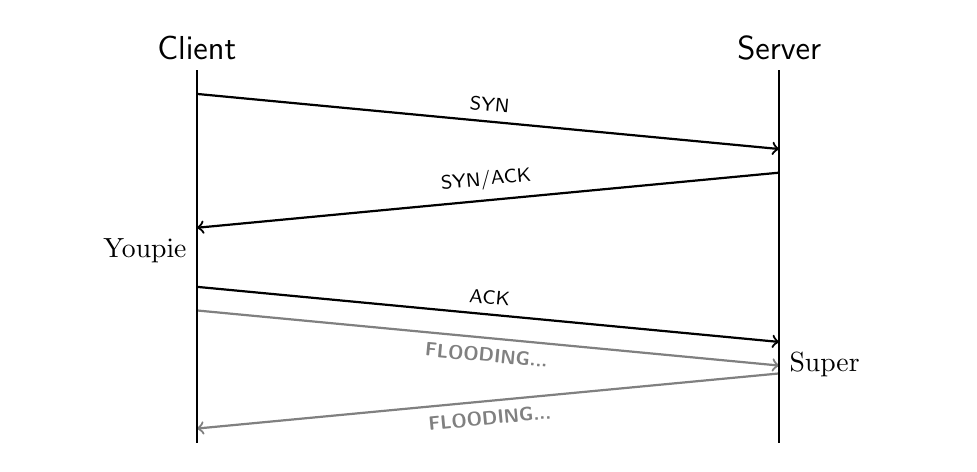
\begin{tikzpicture}[font=\sffamily,thick,
commentl/.style={text width=1.9cm, align=right},
commentr/.style={commentl, align=left},]
\node[] (init) {\large Client};
\node[right=6.1cm of init] (recv) {\large Server};


\draw[->] ([yshift=-0.3cm]init.south) coordinate (syn1o) -- ([yshift=-.7cm]syn1o-|recv) coordinate (syn1e) node[pos=.5, above, sloped] {\scriptsize SYN};

\draw[->] ([yshift=-0.3cm]syn1e) coordinate (synack1o) -- ([yshift=-.7cm]synack1o-|init) coordinate (synack1e) node[pos=.5, above, sloped] {\scriptsize SYN/ACK};

\node[commentl, below left =0mm of synack1e, font=\fontsize{9pt}{9pt}\biolinum]{Youpie};

\draw[->] ([yshift=-.75cm]synack1e) coordinate (ack1o) -- ([yshift=-.7cm]ack1o-|recv) coordinate (ack1e) node[pos=.5, above, sloped] {\scriptsize ACK};

\node[commentr, below right =0mm of ack1e, font=\fontsize{9pt}{9pt}\biolinum]{Super};

%\draw[->] ([yshift=-.4cm]ack1e) coordinate (ack2o) -- ([yshift=-.7cm]ack2o-|init) coordinate (ack2e) node[pos=.5, above, sloped] {\scriptsize ACK};
\draw[gray,->] ([yshift=-.3cm]ack1o) coordinate (data1o) -- ([yshift=-.3cm]ack1e) coordinate (data1e) node[pos=.5, below, sloped] {\scriptsize \textbf{FLOODING...}};

\draw[gray,->] ([yshift=-.4cm]ack1e) coordinate (data2o) -- ([yshift=-.7cm]data2o-|init) coordinate (data2e) node[pos=.5, below, sloped] {\scriptsize \textbf{FLOODING...}};

\node[below =4.5cm of init](end){};

\draw[thick, shorten >=-.1cm] (init) -- (init|-end);
\draw[thick, shorten >=-.1cm] (recv) -- (recv|-end);
\end{tikzpicture}
	\caption{Establishing a \tcp connection.}
	\label{fig:tips:tcp_open_seqdiag}
\end{figure}

\section{Regular Plots}

You can make plots easily with, e.g., \texttt{matplotlib}.
I personally find that PGF files render better than PDF ones, though it is a matter of opinion.

\begin{figure}
	%% Creator: Matplotlib, PGF backend
%%
%% To include the figure in your LaTeX document, write
%%   \input{<filename>.pgf}
%%
%% Make sure the required packages are loaded in your preamble
%%   \usepackage{pgf}
%%
%% Figures using additional raster images can only be included by \input if
%% they are in the same directory as the main LaTeX file. For loading figures
%% from other directories you can use the `import` package
%%   \usepackage{import}
%% and then include the figures with
%%   \import{<path to file>}{<filename>.pgf}
%%
%% Matplotlib used the following preamble
%%
\begingroup%
\makeatletter%
\begin{pgfpicture}%
\pgfpathrectangle{\pgfpointorigin}{\pgfqpoint{4.724409in}{2.919846in}}%
\pgfusepath{use as bounding box, clip}%
\begin{pgfscope}%
\pgfsetbuttcap%
\pgfsetmiterjoin%
\definecolor{currentfill}{rgb}{1.000000,1.000000,1.000000}%
\pgfsetfillcolor{currentfill}%
\pgfsetlinewidth{0.000000pt}%
\definecolor{currentstroke}{rgb}{1.000000,1.000000,1.000000}%
\pgfsetstrokecolor{currentstroke}%
\pgfsetdash{}{0pt}%
\pgfpathmoveto{\pgfqpoint{0.000000in}{0.000000in}}%
\pgfpathlineto{\pgfqpoint{4.724409in}{0.000000in}}%
\pgfpathlineto{\pgfqpoint{4.724409in}{2.919846in}}%
\pgfpathlineto{\pgfqpoint{0.000000in}{2.919846in}}%
\pgfpathclose%
\pgfusepath{fill}%
\end{pgfscope}%
\begin{pgfscope}%
\pgfsetbuttcap%
\pgfsetmiterjoin%
\definecolor{currentfill}{rgb}{1.000000,1.000000,1.000000}%
\pgfsetfillcolor{currentfill}%
\pgfsetlinewidth{0.000000pt}%
\definecolor{currentstroke}{rgb}{0.000000,0.000000,0.000000}%
\pgfsetstrokecolor{currentstroke}%
\pgfsetstrokeopacity{0.000000}%
\pgfsetdash{}{0pt}%
\pgfpathmoveto{\pgfqpoint{0.637966in}{0.612077in}}%
\pgfpathlineto{\pgfqpoint{4.460488in}{0.612077in}}%
\pgfpathlineto{\pgfqpoint{4.460488in}{2.692419in}}%
\pgfpathlineto{\pgfqpoint{0.637966in}{2.692419in}}%
\pgfpathclose%
\pgfusepath{fill}%
\end{pgfscope}%
\begin{pgfscope}%
\pgfpathrectangle{\pgfqpoint{0.637966in}{0.612077in}}{\pgfqpoint{3.822522in}{2.080342in}}%
\pgfusepath{clip}%
\pgfsetrectcap%
\pgfsetroundjoin%
\pgfsetlinewidth{0.803000pt}%
\definecolor{currentstroke}{rgb}{0.690196,0.690196,0.690196}%
\pgfsetstrokecolor{currentstroke}%
\pgfsetstrokeopacity{0.250000}%
\pgfsetdash{}{0pt}%
\pgfpathmoveto{\pgfqpoint{0.637966in}{0.612077in}}%
\pgfpathlineto{\pgfqpoint{0.637966in}{2.692419in}}%
\pgfusepath{stroke}%
\end{pgfscope}%
\begin{pgfscope}%
\pgfsetbuttcap%
\pgfsetroundjoin%
\definecolor{currentfill}{rgb}{0.000000,0.000000,0.000000}%
\pgfsetfillcolor{currentfill}%
\pgfsetlinewidth{0.803000pt}%
\definecolor{currentstroke}{rgb}{0.000000,0.000000,0.000000}%
\pgfsetstrokecolor{currentstroke}%
\pgfsetdash{}{0pt}%
\pgfsys@defobject{currentmarker}{\pgfqpoint{0.000000in}{-0.048611in}}{\pgfqpoint{0.000000in}{0.000000in}}{%
\pgfpathmoveto{\pgfqpoint{0.000000in}{0.000000in}}%
\pgfpathlineto{\pgfqpoint{0.000000in}{-0.048611in}}%
\pgfusepath{stroke,fill}%
}%
\begin{pgfscope}%
\pgfsys@transformshift{0.637966in}{0.612077in}%
\pgfsys@useobject{currentmarker}{}%
\end{pgfscope}%
\end{pgfscope}%
\begin{pgfscope}%
\definecolor{textcolor}{rgb}{0.000000,0.000000,0.000000}%
\pgfsetstrokecolor{textcolor}%
\pgfsetfillcolor{textcolor}%
\pgftext[x=0.637966in,y=0.514855in,,top]{\color{textcolor}\sffamily\fontsize{10.000000}{12.000000}\selectfont \(\displaystyle -2.0\)}%
\end{pgfscope}%
\begin{pgfscope}%
\pgfpathrectangle{\pgfqpoint{0.637966in}{0.612077in}}{\pgfqpoint{3.822522in}{2.080342in}}%
\pgfusepath{clip}%
\pgfsetrectcap%
\pgfsetroundjoin%
\pgfsetlinewidth{0.803000pt}%
\definecolor{currentstroke}{rgb}{0.690196,0.690196,0.690196}%
\pgfsetstrokecolor{currentstroke}%
\pgfsetstrokeopacity{0.250000}%
\pgfsetdash{}{0pt}%
\pgfpathmoveto{\pgfqpoint{1.115781in}{0.612077in}}%
\pgfpathlineto{\pgfqpoint{1.115781in}{2.692419in}}%
\pgfusepath{stroke}%
\end{pgfscope}%
\begin{pgfscope}%
\pgfsetbuttcap%
\pgfsetroundjoin%
\definecolor{currentfill}{rgb}{0.000000,0.000000,0.000000}%
\pgfsetfillcolor{currentfill}%
\pgfsetlinewidth{0.803000pt}%
\definecolor{currentstroke}{rgb}{0.000000,0.000000,0.000000}%
\pgfsetstrokecolor{currentstroke}%
\pgfsetdash{}{0pt}%
\pgfsys@defobject{currentmarker}{\pgfqpoint{0.000000in}{-0.048611in}}{\pgfqpoint{0.000000in}{0.000000in}}{%
\pgfpathmoveto{\pgfqpoint{0.000000in}{0.000000in}}%
\pgfpathlineto{\pgfqpoint{0.000000in}{-0.048611in}}%
\pgfusepath{stroke,fill}%
}%
\begin{pgfscope}%
\pgfsys@transformshift{1.115781in}{0.612077in}%
\pgfsys@useobject{currentmarker}{}%
\end{pgfscope}%
\end{pgfscope}%
\begin{pgfscope}%
\definecolor{textcolor}{rgb}{0.000000,0.000000,0.000000}%
\pgfsetstrokecolor{textcolor}%
\pgfsetfillcolor{textcolor}%
\pgftext[x=1.115781in,y=0.514855in,,top]{\color{textcolor}\sffamily\fontsize{10.000000}{12.000000}\selectfont \(\displaystyle -1.5\)}%
\end{pgfscope}%
\begin{pgfscope}%
\pgfpathrectangle{\pgfqpoint{0.637966in}{0.612077in}}{\pgfqpoint{3.822522in}{2.080342in}}%
\pgfusepath{clip}%
\pgfsetrectcap%
\pgfsetroundjoin%
\pgfsetlinewidth{0.803000pt}%
\definecolor{currentstroke}{rgb}{0.690196,0.690196,0.690196}%
\pgfsetstrokecolor{currentstroke}%
\pgfsetstrokeopacity{0.250000}%
\pgfsetdash{}{0pt}%
\pgfpathmoveto{\pgfqpoint{1.593597in}{0.612077in}}%
\pgfpathlineto{\pgfqpoint{1.593597in}{2.692419in}}%
\pgfusepath{stroke}%
\end{pgfscope}%
\begin{pgfscope}%
\pgfsetbuttcap%
\pgfsetroundjoin%
\definecolor{currentfill}{rgb}{0.000000,0.000000,0.000000}%
\pgfsetfillcolor{currentfill}%
\pgfsetlinewidth{0.803000pt}%
\definecolor{currentstroke}{rgb}{0.000000,0.000000,0.000000}%
\pgfsetstrokecolor{currentstroke}%
\pgfsetdash{}{0pt}%
\pgfsys@defobject{currentmarker}{\pgfqpoint{0.000000in}{-0.048611in}}{\pgfqpoint{0.000000in}{0.000000in}}{%
\pgfpathmoveto{\pgfqpoint{0.000000in}{0.000000in}}%
\pgfpathlineto{\pgfqpoint{0.000000in}{-0.048611in}}%
\pgfusepath{stroke,fill}%
}%
\begin{pgfscope}%
\pgfsys@transformshift{1.593597in}{0.612077in}%
\pgfsys@useobject{currentmarker}{}%
\end{pgfscope}%
\end{pgfscope}%
\begin{pgfscope}%
\definecolor{textcolor}{rgb}{0.000000,0.000000,0.000000}%
\pgfsetstrokecolor{textcolor}%
\pgfsetfillcolor{textcolor}%
\pgftext[x=1.593597in,y=0.514855in,,top]{\color{textcolor}\sffamily\fontsize{10.000000}{12.000000}\selectfont \(\displaystyle -1.0\)}%
\end{pgfscope}%
\begin{pgfscope}%
\pgfpathrectangle{\pgfqpoint{0.637966in}{0.612077in}}{\pgfqpoint{3.822522in}{2.080342in}}%
\pgfusepath{clip}%
\pgfsetrectcap%
\pgfsetroundjoin%
\pgfsetlinewidth{0.803000pt}%
\definecolor{currentstroke}{rgb}{0.690196,0.690196,0.690196}%
\pgfsetstrokecolor{currentstroke}%
\pgfsetstrokeopacity{0.250000}%
\pgfsetdash{}{0pt}%
\pgfpathmoveto{\pgfqpoint{2.071412in}{0.612077in}}%
\pgfpathlineto{\pgfqpoint{2.071412in}{2.692419in}}%
\pgfusepath{stroke}%
\end{pgfscope}%
\begin{pgfscope}%
\pgfsetbuttcap%
\pgfsetroundjoin%
\definecolor{currentfill}{rgb}{0.000000,0.000000,0.000000}%
\pgfsetfillcolor{currentfill}%
\pgfsetlinewidth{0.803000pt}%
\definecolor{currentstroke}{rgb}{0.000000,0.000000,0.000000}%
\pgfsetstrokecolor{currentstroke}%
\pgfsetdash{}{0pt}%
\pgfsys@defobject{currentmarker}{\pgfqpoint{0.000000in}{-0.048611in}}{\pgfqpoint{0.000000in}{0.000000in}}{%
\pgfpathmoveto{\pgfqpoint{0.000000in}{0.000000in}}%
\pgfpathlineto{\pgfqpoint{0.000000in}{-0.048611in}}%
\pgfusepath{stroke,fill}%
}%
\begin{pgfscope}%
\pgfsys@transformshift{2.071412in}{0.612077in}%
\pgfsys@useobject{currentmarker}{}%
\end{pgfscope}%
\end{pgfscope}%
\begin{pgfscope}%
\definecolor{textcolor}{rgb}{0.000000,0.000000,0.000000}%
\pgfsetstrokecolor{textcolor}%
\pgfsetfillcolor{textcolor}%
\pgftext[x=2.071412in,y=0.514855in,,top]{\color{textcolor}\sffamily\fontsize{10.000000}{12.000000}\selectfont \(\displaystyle -0.5\)}%
\end{pgfscope}%
\begin{pgfscope}%
\pgfpathrectangle{\pgfqpoint{0.637966in}{0.612077in}}{\pgfqpoint{3.822522in}{2.080342in}}%
\pgfusepath{clip}%
\pgfsetrectcap%
\pgfsetroundjoin%
\pgfsetlinewidth{0.803000pt}%
\definecolor{currentstroke}{rgb}{0.690196,0.690196,0.690196}%
\pgfsetstrokecolor{currentstroke}%
\pgfsetstrokeopacity{0.250000}%
\pgfsetdash{}{0pt}%
\pgfpathmoveto{\pgfqpoint{2.549227in}{0.612077in}}%
\pgfpathlineto{\pgfqpoint{2.549227in}{2.692419in}}%
\pgfusepath{stroke}%
\end{pgfscope}%
\begin{pgfscope}%
\pgfsetbuttcap%
\pgfsetroundjoin%
\definecolor{currentfill}{rgb}{0.000000,0.000000,0.000000}%
\pgfsetfillcolor{currentfill}%
\pgfsetlinewidth{0.803000pt}%
\definecolor{currentstroke}{rgb}{0.000000,0.000000,0.000000}%
\pgfsetstrokecolor{currentstroke}%
\pgfsetdash{}{0pt}%
\pgfsys@defobject{currentmarker}{\pgfqpoint{0.000000in}{-0.048611in}}{\pgfqpoint{0.000000in}{0.000000in}}{%
\pgfpathmoveto{\pgfqpoint{0.000000in}{0.000000in}}%
\pgfpathlineto{\pgfqpoint{0.000000in}{-0.048611in}}%
\pgfusepath{stroke,fill}%
}%
\begin{pgfscope}%
\pgfsys@transformshift{2.549227in}{0.612077in}%
\pgfsys@useobject{currentmarker}{}%
\end{pgfscope}%
\end{pgfscope}%
\begin{pgfscope}%
\definecolor{textcolor}{rgb}{0.000000,0.000000,0.000000}%
\pgfsetstrokecolor{textcolor}%
\pgfsetfillcolor{textcolor}%
\pgftext[x=2.549227in,y=0.514855in,,top]{\color{textcolor}\sffamily\fontsize{10.000000}{12.000000}\selectfont \(\displaystyle 0.0\)}%
\end{pgfscope}%
\begin{pgfscope}%
\pgfpathrectangle{\pgfqpoint{0.637966in}{0.612077in}}{\pgfqpoint{3.822522in}{2.080342in}}%
\pgfusepath{clip}%
\pgfsetrectcap%
\pgfsetroundjoin%
\pgfsetlinewidth{0.803000pt}%
\definecolor{currentstroke}{rgb}{0.690196,0.690196,0.690196}%
\pgfsetstrokecolor{currentstroke}%
\pgfsetstrokeopacity{0.250000}%
\pgfsetdash{}{0pt}%
\pgfpathmoveto{\pgfqpoint{3.027042in}{0.612077in}}%
\pgfpathlineto{\pgfqpoint{3.027042in}{2.692419in}}%
\pgfusepath{stroke}%
\end{pgfscope}%
\begin{pgfscope}%
\pgfsetbuttcap%
\pgfsetroundjoin%
\definecolor{currentfill}{rgb}{0.000000,0.000000,0.000000}%
\pgfsetfillcolor{currentfill}%
\pgfsetlinewidth{0.803000pt}%
\definecolor{currentstroke}{rgb}{0.000000,0.000000,0.000000}%
\pgfsetstrokecolor{currentstroke}%
\pgfsetdash{}{0pt}%
\pgfsys@defobject{currentmarker}{\pgfqpoint{0.000000in}{-0.048611in}}{\pgfqpoint{0.000000in}{0.000000in}}{%
\pgfpathmoveto{\pgfqpoint{0.000000in}{0.000000in}}%
\pgfpathlineto{\pgfqpoint{0.000000in}{-0.048611in}}%
\pgfusepath{stroke,fill}%
}%
\begin{pgfscope}%
\pgfsys@transformshift{3.027042in}{0.612077in}%
\pgfsys@useobject{currentmarker}{}%
\end{pgfscope}%
\end{pgfscope}%
\begin{pgfscope}%
\definecolor{textcolor}{rgb}{0.000000,0.000000,0.000000}%
\pgfsetstrokecolor{textcolor}%
\pgfsetfillcolor{textcolor}%
\pgftext[x=3.027042in,y=0.514855in,,top]{\color{textcolor}\sffamily\fontsize{10.000000}{12.000000}\selectfont \(\displaystyle 0.5\)}%
\end{pgfscope}%
\begin{pgfscope}%
\pgfpathrectangle{\pgfqpoint{0.637966in}{0.612077in}}{\pgfqpoint{3.822522in}{2.080342in}}%
\pgfusepath{clip}%
\pgfsetrectcap%
\pgfsetroundjoin%
\pgfsetlinewidth{0.803000pt}%
\definecolor{currentstroke}{rgb}{0.690196,0.690196,0.690196}%
\pgfsetstrokecolor{currentstroke}%
\pgfsetstrokeopacity{0.250000}%
\pgfsetdash{}{0pt}%
\pgfpathmoveto{\pgfqpoint{3.504858in}{0.612077in}}%
\pgfpathlineto{\pgfqpoint{3.504858in}{2.692419in}}%
\pgfusepath{stroke}%
\end{pgfscope}%
\begin{pgfscope}%
\pgfsetbuttcap%
\pgfsetroundjoin%
\definecolor{currentfill}{rgb}{0.000000,0.000000,0.000000}%
\pgfsetfillcolor{currentfill}%
\pgfsetlinewidth{0.803000pt}%
\definecolor{currentstroke}{rgb}{0.000000,0.000000,0.000000}%
\pgfsetstrokecolor{currentstroke}%
\pgfsetdash{}{0pt}%
\pgfsys@defobject{currentmarker}{\pgfqpoint{0.000000in}{-0.048611in}}{\pgfqpoint{0.000000in}{0.000000in}}{%
\pgfpathmoveto{\pgfqpoint{0.000000in}{0.000000in}}%
\pgfpathlineto{\pgfqpoint{0.000000in}{-0.048611in}}%
\pgfusepath{stroke,fill}%
}%
\begin{pgfscope}%
\pgfsys@transformshift{3.504858in}{0.612077in}%
\pgfsys@useobject{currentmarker}{}%
\end{pgfscope}%
\end{pgfscope}%
\begin{pgfscope}%
\definecolor{textcolor}{rgb}{0.000000,0.000000,0.000000}%
\pgfsetstrokecolor{textcolor}%
\pgfsetfillcolor{textcolor}%
\pgftext[x=3.504858in,y=0.514855in,,top]{\color{textcolor}\sffamily\fontsize{10.000000}{12.000000}\selectfont \(\displaystyle 1.0\)}%
\end{pgfscope}%
\begin{pgfscope}%
\pgfpathrectangle{\pgfqpoint{0.637966in}{0.612077in}}{\pgfqpoint{3.822522in}{2.080342in}}%
\pgfusepath{clip}%
\pgfsetrectcap%
\pgfsetroundjoin%
\pgfsetlinewidth{0.803000pt}%
\definecolor{currentstroke}{rgb}{0.690196,0.690196,0.690196}%
\pgfsetstrokecolor{currentstroke}%
\pgfsetstrokeopacity{0.250000}%
\pgfsetdash{}{0pt}%
\pgfpathmoveto{\pgfqpoint{3.982673in}{0.612077in}}%
\pgfpathlineto{\pgfqpoint{3.982673in}{2.692419in}}%
\pgfusepath{stroke}%
\end{pgfscope}%
\begin{pgfscope}%
\pgfsetbuttcap%
\pgfsetroundjoin%
\definecolor{currentfill}{rgb}{0.000000,0.000000,0.000000}%
\pgfsetfillcolor{currentfill}%
\pgfsetlinewidth{0.803000pt}%
\definecolor{currentstroke}{rgb}{0.000000,0.000000,0.000000}%
\pgfsetstrokecolor{currentstroke}%
\pgfsetdash{}{0pt}%
\pgfsys@defobject{currentmarker}{\pgfqpoint{0.000000in}{-0.048611in}}{\pgfqpoint{0.000000in}{0.000000in}}{%
\pgfpathmoveto{\pgfqpoint{0.000000in}{0.000000in}}%
\pgfpathlineto{\pgfqpoint{0.000000in}{-0.048611in}}%
\pgfusepath{stroke,fill}%
}%
\begin{pgfscope}%
\pgfsys@transformshift{3.982673in}{0.612077in}%
\pgfsys@useobject{currentmarker}{}%
\end{pgfscope}%
\end{pgfscope}%
\begin{pgfscope}%
\definecolor{textcolor}{rgb}{0.000000,0.000000,0.000000}%
\pgfsetstrokecolor{textcolor}%
\pgfsetfillcolor{textcolor}%
\pgftext[x=3.982673in,y=0.514855in,,top]{\color{textcolor}\sffamily\fontsize{10.000000}{12.000000}\selectfont \(\displaystyle 1.5\)}%
\end{pgfscope}%
\begin{pgfscope}%
\pgfpathrectangle{\pgfqpoint{0.637966in}{0.612077in}}{\pgfqpoint{3.822522in}{2.080342in}}%
\pgfusepath{clip}%
\pgfsetrectcap%
\pgfsetroundjoin%
\pgfsetlinewidth{0.803000pt}%
\definecolor{currentstroke}{rgb}{0.690196,0.690196,0.690196}%
\pgfsetstrokecolor{currentstroke}%
\pgfsetstrokeopacity{0.250000}%
\pgfsetdash{}{0pt}%
\pgfpathmoveto{\pgfqpoint{4.460488in}{0.612077in}}%
\pgfpathlineto{\pgfqpoint{4.460488in}{2.692419in}}%
\pgfusepath{stroke}%
\end{pgfscope}%
\begin{pgfscope}%
\pgfsetbuttcap%
\pgfsetroundjoin%
\definecolor{currentfill}{rgb}{0.000000,0.000000,0.000000}%
\pgfsetfillcolor{currentfill}%
\pgfsetlinewidth{0.803000pt}%
\definecolor{currentstroke}{rgb}{0.000000,0.000000,0.000000}%
\pgfsetstrokecolor{currentstroke}%
\pgfsetdash{}{0pt}%
\pgfsys@defobject{currentmarker}{\pgfqpoint{0.000000in}{-0.048611in}}{\pgfqpoint{0.000000in}{0.000000in}}{%
\pgfpathmoveto{\pgfqpoint{0.000000in}{0.000000in}}%
\pgfpathlineto{\pgfqpoint{0.000000in}{-0.048611in}}%
\pgfusepath{stroke,fill}%
}%
\begin{pgfscope}%
\pgfsys@transformshift{4.460488in}{0.612077in}%
\pgfsys@useobject{currentmarker}{}%
\end{pgfscope}%
\end{pgfscope}%
\begin{pgfscope}%
\definecolor{textcolor}{rgb}{0.000000,0.000000,0.000000}%
\pgfsetstrokecolor{textcolor}%
\pgfsetfillcolor{textcolor}%
\pgftext[x=4.460488in,y=0.514855in,,top]{\color{textcolor}\sffamily\fontsize{10.000000}{12.000000}\selectfont \(\displaystyle 2.0\)}%
\end{pgfscope}%
\begin{pgfscope}%
\definecolor{textcolor}{rgb}{0.000000,0.000000,0.000000}%
\pgfsetstrokecolor{textcolor}%
\pgfsetfillcolor{textcolor}%
\pgftext[x=2.549227in,y=0.335843in,,top]{\color{textcolor}\sffamily\fontsize{12.000000}{14.400000}\selectfont \(\displaystyle x\) value}%
\end{pgfscope}%
\begin{pgfscope}%
\pgfpathrectangle{\pgfqpoint{0.637966in}{0.612077in}}{\pgfqpoint{3.822522in}{2.080342in}}%
\pgfusepath{clip}%
\pgfsetrectcap%
\pgfsetroundjoin%
\pgfsetlinewidth{0.803000pt}%
\definecolor{currentstroke}{rgb}{0.690196,0.690196,0.690196}%
\pgfsetstrokecolor{currentstroke}%
\pgfsetstrokeopacity{0.250000}%
\pgfsetdash{}{0pt}%
\pgfpathmoveto{\pgfqpoint{0.637966in}{0.677088in}}%
\pgfpathlineto{\pgfqpoint{4.460488in}{0.677088in}}%
\pgfusepath{stroke}%
\end{pgfscope}%
\begin{pgfscope}%
\pgfsetbuttcap%
\pgfsetroundjoin%
\definecolor{currentfill}{rgb}{0.000000,0.000000,0.000000}%
\pgfsetfillcolor{currentfill}%
\pgfsetlinewidth{0.803000pt}%
\definecolor{currentstroke}{rgb}{0.000000,0.000000,0.000000}%
\pgfsetstrokecolor{currentstroke}%
\pgfsetdash{}{0pt}%
\pgfsys@defobject{currentmarker}{\pgfqpoint{-0.048611in}{0.000000in}}{\pgfqpoint{0.000000in}{0.000000in}}{%
\pgfpathmoveto{\pgfqpoint{0.000000in}{0.000000in}}%
\pgfpathlineto{\pgfqpoint{-0.048611in}{0.000000in}}%
\pgfusepath{stroke,fill}%
}%
\begin{pgfscope}%
\pgfsys@transformshift{0.637966in}{0.677088in}%
\pgfsys@useobject{currentmarker}{}%
\end{pgfscope}%
\end{pgfscope}%
\begin{pgfscope}%
\definecolor{textcolor}{rgb}{0.000000,0.000000,0.000000}%
\pgfsetstrokecolor{textcolor}%
\pgfsetfillcolor{textcolor}%
\pgftext[x=0.255249in,y=0.628863in,left,base]{\color{textcolor}\sffamily\fontsize{10.000000}{12.000000}\selectfont \(\displaystyle -7.5\)}%
\end{pgfscope}%
\begin{pgfscope}%
\pgfpathrectangle{\pgfqpoint{0.637966in}{0.612077in}}{\pgfqpoint{3.822522in}{2.080342in}}%
\pgfusepath{clip}%
\pgfsetrectcap%
\pgfsetroundjoin%
\pgfsetlinewidth{0.803000pt}%
\definecolor{currentstroke}{rgb}{0.690196,0.690196,0.690196}%
\pgfsetstrokecolor{currentstroke}%
\pgfsetstrokeopacity{0.250000}%
\pgfsetdash{}{0pt}%
\pgfpathmoveto{\pgfqpoint{0.637966in}{1.002141in}}%
\pgfpathlineto{\pgfqpoint{4.460488in}{1.002141in}}%
\pgfusepath{stroke}%
\end{pgfscope}%
\begin{pgfscope}%
\pgfsetbuttcap%
\pgfsetroundjoin%
\definecolor{currentfill}{rgb}{0.000000,0.000000,0.000000}%
\pgfsetfillcolor{currentfill}%
\pgfsetlinewidth{0.803000pt}%
\definecolor{currentstroke}{rgb}{0.000000,0.000000,0.000000}%
\pgfsetstrokecolor{currentstroke}%
\pgfsetdash{}{0pt}%
\pgfsys@defobject{currentmarker}{\pgfqpoint{-0.048611in}{0.000000in}}{\pgfqpoint{0.000000in}{0.000000in}}{%
\pgfpathmoveto{\pgfqpoint{0.000000in}{0.000000in}}%
\pgfpathlineto{\pgfqpoint{-0.048611in}{0.000000in}}%
\pgfusepath{stroke,fill}%
}%
\begin{pgfscope}%
\pgfsys@transformshift{0.637966in}{1.002141in}%
\pgfsys@useobject{currentmarker}{}%
\end{pgfscope}%
\end{pgfscope}%
\begin{pgfscope}%
\definecolor{textcolor}{rgb}{0.000000,0.000000,0.000000}%
\pgfsetstrokecolor{textcolor}%
\pgfsetfillcolor{textcolor}%
\pgftext[x=0.255249in,y=0.953916in,left,base]{\color{textcolor}\sffamily\fontsize{10.000000}{12.000000}\selectfont \(\displaystyle -5.0\)}%
\end{pgfscope}%
\begin{pgfscope}%
\pgfpathrectangle{\pgfqpoint{0.637966in}{0.612077in}}{\pgfqpoint{3.822522in}{2.080342in}}%
\pgfusepath{clip}%
\pgfsetrectcap%
\pgfsetroundjoin%
\pgfsetlinewidth{0.803000pt}%
\definecolor{currentstroke}{rgb}{0.690196,0.690196,0.690196}%
\pgfsetstrokecolor{currentstroke}%
\pgfsetstrokeopacity{0.250000}%
\pgfsetdash{}{0pt}%
\pgfpathmoveto{\pgfqpoint{0.637966in}{1.327195in}}%
\pgfpathlineto{\pgfqpoint{4.460488in}{1.327195in}}%
\pgfusepath{stroke}%
\end{pgfscope}%
\begin{pgfscope}%
\pgfsetbuttcap%
\pgfsetroundjoin%
\definecolor{currentfill}{rgb}{0.000000,0.000000,0.000000}%
\pgfsetfillcolor{currentfill}%
\pgfsetlinewidth{0.803000pt}%
\definecolor{currentstroke}{rgb}{0.000000,0.000000,0.000000}%
\pgfsetstrokecolor{currentstroke}%
\pgfsetdash{}{0pt}%
\pgfsys@defobject{currentmarker}{\pgfqpoint{-0.048611in}{0.000000in}}{\pgfqpoint{0.000000in}{0.000000in}}{%
\pgfpathmoveto{\pgfqpoint{0.000000in}{0.000000in}}%
\pgfpathlineto{\pgfqpoint{-0.048611in}{0.000000in}}%
\pgfusepath{stroke,fill}%
}%
\begin{pgfscope}%
\pgfsys@transformshift{0.637966in}{1.327195in}%
\pgfsys@useobject{currentmarker}{}%
\end{pgfscope}%
\end{pgfscope}%
\begin{pgfscope}%
\definecolor{textcolor}{rgb}{0.000000,0.000000,0.000000}%
\pgfsetstrokecolor{textcolor}%
\pgfsetfillcolor{textcolor}%
\pgftext[x=0.255249in,y=1.278970in,left,base]{\color{textcolor}\sffamily\fontsize{10.000000}{12.000000}\selectfont \(\displaystyle -2.5\)}%
\end{pgfscope}%
\begin{pgfscope}%
\pgfpathrectangle{\pgfqpoint{0.637966in}{0.612077in}}{\pgfqpoint{3.822522in}{2.080342in}}%
\pgfusepath{clip}%
\pgfsetrectcap%
\pgfsetroundjoin%
\pgfsetlinewidth{0.803000pt}%
\definecolor{currentstroke}{rgb}{0.690196,0.690196,0.690196}%
\pgfsetstrokecolor{currentstroke}%
\pgfsetstrokeopacity{0.250000}%
\pgfsetdash{}{0pt}%
\pgfpathmoveto{\pgfqpoint{0.637966in}{1.652248in}}%
\pgfpathlineto{\pgfqpoint{4.460488in}{1.652248in}}%
\pgfusepath{stroke}%
\end{pgfscope}%
\begin{pgfscope}%
\pgfsetbuttcap%
\pgfsetroundjoin%
\definecolor{currentfill}{rgb}{0.000000,0.000000,0.000000}%
\pgfsetfillcolor{currentfill}%
\pgfsetlinewidth{0.803000pt}%
\definecolor{currentstroke}{rgb}{0.000000,0.000000,0.000000}%
\pgfsetstrokecolor{currentstroke}%
\pgfsetdash{}{0pt}%
\pgfsys@defobject{currentmarker}{\pgfqpoint{-0.048611in}{0.000000in}}{\pgfqpoint{0.000000in}{0.000000in}}{%
\pgfpathmoveto{\pgfqpoint{0.000000in}{0.000000in}}%
\pgfpathlineto{\pgfqpoint{-0.048611in}{0.000000in}}%
\pgfusepath{stroke,fill}%
}%
\begin{pgfscope}%
\pgfsys@transformshift{0.637966in}{1.652248in}%
\pgfsys@useobject{currentmarker}{}%
\end{pgfscope}%
\end{pgfscope}%
\begin{pgfscope}%
\definecolor{textcolor}{rgb}{0.000000,0.000000,0.000000}%
\pgfsetstrokecolor{textcolor}%
\pgfsetfillcolor{textcolor}%
\pgftext[x=0.363274in,y=1.604023in,left,base]{\color{textcolor}\sffamily\fontsize{10.000000}{12.000000}\selectfont \(\displaystyle 0.0\)}%
\end{pgfscope}%
\begin{pgfscope}%
\pgfpathrectangle{\pgfqpoint{0.637966in}{0.612077in}}{\pgfqpoint{3.822522in}{2.080342in}}%
\pgfusepath{clip}%
\pgfsetrectcap%
\pgfsetroundjoin%
\pgfsetlinewidth{0.803000pt}%
\definecolor{currentstroke}{rgb}{0.690196,0.690196,0.690196}%
\pgfsetstrokecolor{currentstroke}%
\pgfsetstrokeopacity{0.250000}%
\pgfsetdash{}{0pt}%
\pgfpathmoveto{\pgfqpoint{0.637966in}{1.977302in}}%
\pgfpathlineto{\pgfqpoint{4.460488in}{1.977302in}}%
\pgfusepath{stroke}%
\end{pgfscope}%
\begin{pgfscope}%
\pgfsetbuttcap%
\pgfsetroundjoin%
\definecolor{currentfill}{rgb}{0.000000,0.000000,0.000000}%
\pgfsetfillcolor{currentfill}%
\pgfsetlinewidth{0.803000pt}%
\definecolor{currentstroke}{rgb}{0.000000,0.000000,0.000000}%
\pgfsetstrokecolor{currentstroke}%
\pgfsetdash{}{0pt}%
\pgfsys@defobject{currentmarker}{\pgfqpoint{-0.048611in}{0.000000in}}{\pgfqpoint{0.000000in}{0.000000in}}{%
\pgfpathmoveto{\pgfqpoint{0.000000in}{0.000000in}}%
\pgfpathlineto{\pgfqpoint{-0.048611in}{0.000000in}}%
\pgfusepath{stroke,fill}%
}%
\begin{pgfscope}%
\pgfsys@transformshift{0.637966in}{1.977302in}%
\pgfsys@useobject{currentmarker}{}%
\end{pgfscope}%
\end{pgfscope}%
\begin{pgfscope}%
\definecolor{textcolor}{rgb}{0.000000,0.000000,0.000000}%
\pgfsetstrokecolor{textcolor}%
\pgfsetfillcolor{textcolor}%
\pgftext[x=0.363274in,y=1.929076in,left,base]{\color{textcolor}\sffamily\fontsize{10.000000}{12.000000}\selectfont \(\displaystyle 2.5\)}%
\end{pgfscope}%
\begin{pgfscope}%
\pgfpathrectangle{\pgfqpoint{0.637966in}{0.612077in}}{\pgfqpoint{3.822522in}{2.080342in}}%
\pgfusepath{clip}%
\pgfsetrectcap%
\pgfsetroundjoin%
\pgfsetlinewidth{0.803000pt}%
\definecolor{currentstroke}{rgb}{0.690196,0.690196,0.690196}%
\pgfsetstrokecolor{currentstroke}%
\pgfsetstrokeopacity{0.250000}%
\pgfsetdash{}{0pt}%
\pgfpathmoveto{\pgfqpoint{0.637966in}{2.302355in}}%
\pgfpathlineto{\pgfqpoint{4.460488in}{2.302355in}}%
\pgfusepath{stroke}%
\end{pgfscope}%
\begin{pgfscope}%
\pgfsetbuttcap%
\pgfsetroundjoin%
\definecolor{currentfill}{rgb}{0.000000,0.000000,0.000000}%
\pgfsetfillcolor{currentfill}%
\pgfsetlinewidth{0.803000pt}%
\definecolor{currentstroke}{rgb}{0.000000,0.000000,0.000000}%
\pgfsetstrokecolor{currentstroke}%
\pgfsetdash{}{0pt}%
\pgfsys@defobject{currentmarker}{\pgfqpoint{-0.048611in}{0.000000in}}{\pgfqpoint{0.000000in}{0.000000in}}{%
\pgfpathmoveto{\pgfqpoint{0.000000in}{0.000000in}}%
\pgfpathlineto{\pgfqpoint{-0.048611in}{0.000000in}}%
\pgfusepath{stroke,fill}%
}%
\begin{pgfscope}%
\pgfsys@transformshift{0.637966in}{2.302355in}%
\pgfsys@useobject{currentmarker}{}%
\end{pgfscope}%
\end{pgfscope}%
\begin{pgfscope}%
\definecolor{textcolor}{rgb}{0.000000,0.000000,0.000000}%
\pgfsetstrokecolor{textcolor}%
\pgfsetfillcolor{textcolor}%
\pgftext[x=0.363274in,y=2.254130in,left,base]{\color{textcolor}\sffamily\fontsize{10.000000}{12.000000}\selectfont \(\displaystyle 5.0\)}%
\end{pgfscope}%
\begin{pgfscope}%
\pgfpathrectangle{\pgfqpoint{0.637966in}{0.612077in}}{\pgfqpoint{3.822522in}{2.080342in}}%
\pgfusepath{clip}%
\pgfsetrectcap%
\pgfsetroundjoin%
\pgfsetlinewidth{0.803000pt}%
\definecolor{currentstroke}{rgb}{0.690196,0.690196,0.690196}%
\pgfsetstrokecolor{currentstroke}%
\pgfsetstrokeopacity{0.250000}%
\pgfsetdash{}{0pt}%
\pgfpathmoveto{\pgfqpoint{0.637966in}{2.627409in}}%
\pgfpathlineto{\pgfqpoint{4.460488in}{2.627409in}}%
\pgfusepath{stroke}%
\end{pgfscope}%
\begin{pgfscope}%
\pgfsetbuttcap%
\pgfsetroundjoin%
\definecolor{currentfill}{rgb}{0.000000,0.000000,0.000000}%
\pgfsetfillcolor{currentfill}%
\pgfsetlinewidth{0.803000pt}%
\definecolor{currentstroke}{rgb}{0.000000,0.000000,0.000000}%
\pgfsetstrokecolor{currentstroke}%
\pgfsetdash{}{0pt}%
\pgfsys@defobject{currentmarker}{\pgfqpoint{-0.048611in}{0.000000in}}{\pgfqpoint{0.000000in}{0.000000in}}{%
\pgfpathmoveto{\pgfqpoint{0.000000in}{0.000000in}}%
\pgfpathlineto{\pgfqpoint{-0.048611in}{0.000000in}}%
\pgfusepath{stroke,fill}%
}%
\begin{pgfscope}%
\pgfsys@transformshift{0.637966in}{2.627409in}%
\pgfsys@useobject{currentmarker}{}%
\end{pgfscope}%
\end{pgfscope}%
\begin{pgfscope}%
\definecolor{textcolor}{rgb}{0.000000,0.000000,0.000000}%
\pgfsetstrokecolor{textcolor}%
\pgfsetfillcolor{textcolor}%
\pgftext[x=0.363274in,y=2.579183in,left,base]{\color{textcolor}\sffamily\fontsize{10.000000}{12.000000}\selectfont \(\displaystyle 7.5\)}%
\end{pgfscope}%
\begin{pgfscope}%
\definecolor{textcolor}{rgb}{0.000000,0.000000,0.000000}%
\pgfsetstrokecolor{textcolor}%
\pgfsetfillcolor{textcolor}%
\pgftext[x=0.199694in,y=1.652248in,,bottom,rotate=90.000000]{\color{textcolor}\sffamily\fontsize{12.000000}{14.400000}\selectfont \(\displaystyle y\) value}%
\end{pgfscope}%
\begin{pgfscope}%
\pgfpathrectangle{\pgfqpoint{0.637966in}{0.612077in}}{\pgfqpoint{3.822522in}{2.080342in}}%
\pgfusepath{clip}%
\pgfsetrectcap%
\pgfsetroundjoin%
\pgfsetlinewidth{1.505625pt}%
\definecolor{currentstroke}{rgb}{0.749020,0.749020,0.749020}%
\pgfsetstrokecolor{currentstroke}%
\pgfsetdash{}{0pt}%
\pgfpathmoveto{\pgfqpoint{0.637966in}{2.172334in}}%
\pgfpathlineto{\pgfqpoint{0.753218in}{2.111501in}}%
\pgfpathlineto{\pgfqpoint{0.868470in}{2.054451in}}%
\pgfpathlineto{\pgfqpoint{0.983722in}{2.001183in}}%
\pgfpathlineto{\pgfqpoint{1.098974in}{1.951697in}}%
\pgfpathlineto{\pgfqpoint{1.214226in}{1.905994in}}%
\pgfpathlineto{\pgfqpoint{1.329478in}{1.864073in}}%
\pgfpathlineto{\pgfqpoint{1.444730in}{1.825934in}}%
\pgfpathlineto{\pgfqpoint{1.559982in}{1.791578in}}%
\pgfpathlineto{\pgfqpoint{1.675233in}{1.761004in}}%
\pgfpathlineto{\pgfqpoint{1.790485in}{1.734212in}}%
\pgfpathlineto{\pgfqpoint{1.905737in}{1.711203in}}%
\pgfpathlineto{\pgfqpoint{2.001781in}{1.694918in}}%
\pgfpathlineto{\pgfqpoint{2.097824in}{1.681259in}}%
\pgfpathlineto{\pgfqpoint{2.193867in}{1.670228in}}%
\pgfpathlineto{\pgfqpoint{2.289910in}{1.661822in}}%
\pgfpathlineto{\pgfqpoint{2.385954in}{1.656044in}}%
\pgfpathlineto{\pgfqpoint{2.481997in}{1.652892in}}%
\pgfpathlineto{\pgfqpoint{2.578040in}{1.652366in}}%
\pgfpathlineto{\pgfqpoint{2.674083in}{1.654468in}}%
\pgfpathlineto{\pgfqpoint{2.770127in}{1.659196in}}%
\pgfpathlineto{\pgfqpoint{2.866170in}{1.666550in}}%
\pgfpathlineto{\pgfqpoint{2.962213in}{1.676531in}}%
\pgfpathlineto{\pgfqpoint{3.058257in}{1.689139in}}%
\pgfpathlineto{\pgfqpoint{3.154300in}{1.704374in}}%
\pgfpathlineto{\pgfqpoint{3.250343in}{1.722235in}}%
\pgfpathlineto{\pgfqpoint{3.346386in}{1.742722in}}%
\pgfpathlineto{\pgfqpoint{3.461638in}{1.770775in}}%
\pgfpathlineto{\pgfqpoint{3.576890in}{1.802610in}}%
\pgfpathlineto{\pgfqpoint{3.692142in}{1.838227in}}%
\pgfpathlineto{\pgfqpoint{3.807394in}{1.877626in}}%
\pgfpathlineto{\pgfqpoint{3.922646in}{1.920808in}}%
\pgfpathlineto{\pgfqpoint{4.037898in}{1.967772in}}%
\pgfpathlineto{\pgfqpoint{4.153150in}{2.018518in}}%
\pgfpathlineto{\pgfqpoint{4.268402in}{2.073047in}}%
\pgfpathlineto{\pgfqpoint{4.383654in}{2.131358in}}%
\pgfpathlineto{\pgfqpoint{4.460488in}{2.172334in}}%
\pgfpathlineto{\pgfqpoint{4.460488in}{2.172334in}}%
\pgfusepath{stroke}%
\end{pgfscope}%
\begin{pgfscope}%
\pgfpathrectangle{\pgfqpoint{0.637966in}{0.612077in}}{\pgfqpoint{3.822522in}{2.080342in}}%
\pgfusepath{clip}%
\pgfsetbuttcap%
\pgfsetroundjoin%
\pgfsetlinewidth{1.505625pt}%
\definecolor{currentstroke}{rgb}{0.000000,0.000000,0.000000}%
\pgfsetstrokecolor{currentstroke}%
\pgfsetdash{{5.550000pt}{2.400000pt}}{0.000000pt}%
\pgfpathmoveto{\pgfqpoint{0.637966in}{0.612077in}}%
\pgfpathlineto{\pgfqpoint{0.695592in}{0.703355in}}%
\pgfpathlineto{\pgfqpoint{0.753218in}{0.789130in}}%
\pgfpathlineto{\pgfqpoint{0.810844in}{0.869574in}}%
\pgfpathlineto{\pgfqpoint{0.868470in}{0.944857in}}%
\pgfpathlineto{\pgfqpoint{0.926096in}{1.015151in}}%
\pgfpathlineto{\pgfqpoint{0.983722in}{1.080627in}}%
\pgfpathlineto{\pgfqpoint{1.041348in}{1.141456in}}%
\pgfpathlineto{\pgfqpoint{1.098974in}{1.197808in}}%
\pgfpathlineto{\pgfqpoint{1.156600in}{1.249856in}}%
\pgfpathlineto{\pgfqpoint{1.214226in}{1.297770in}}%
\pgfpathlineto{\pgfqpoint{1.271852in}{1.341720in}}%
\pgfpathlineto{\pgfqpoint{1.329478in}{1.381879in}}%
\pgfpathlineto{\pgfqpoint{1.387104in}{1.418417in}}%
\pgfpathlineto{\pgfqpoint{1.444730in}{1.451506in}}%
\pgfpathlineto{\pgfqpoint{1.502356in}{1.481316in}}%
\pgfpathlineto{\pgfqpoint{1.559982in}{1.508018in}}%
\pgfpathlineto{\pgfqpoint{1.617608in}{1.531783in}}%
\pgfpathlineto{\pgfqpoint{1.675233in}{1.552783in}}%
\pgfpathlineto{\pgfqpoint{1.732859in}{1.571189in}}%
\pgfpathlineto{\pgfqpoint{1.809694in}{1.591990in}}%
\pgfpathlineto{\pgfqpoint{1.886529in}{1.608888in}}%
\pgfpathlineto{\pgfqpoint{1.963363in}{1.622289in}}%
\pgfpathlineto{\pgfqpoint{2.040198in}{1.632598in}}%
\pgfpathlineto{\pgfqpoint{2.136241in}{1.641754in}}%
\pgfpathlineto{\pgfqpoint{2.232284in}{1.647505in}}%
\pgfpathlineto{\pgfqpoint{2.347536in}{1.651026in}}%
\pgfpathlineto{\pgfqpoint{2.501206in}{1.652232in}}%
\pgfpathlineto{\pgfqpoint{2.770127in}{1.653854in}}%
\pgfpathlineto{\pgfqpoint{2.885379in}{1.657907in}}%
\pgfpathlineto{\pgfqpoint{2.981422in}{1.664276in}}%
\pgfpathlineto{\pgfqpoint{3.058257in}{1.671899in}}%
\pgfpathlineto{\pgfqpoint{3.135091in}{1.682208in}}%
\pgfpathlineto{\pgfqpoint{3.211926in}{1.695609in}}%
\pgfpathlineto{\pgfqpoint{3.288760in}{1.712507in}}%
\pgfpathlineto{\pgfqpoint{3.365595in}{1.733307in}}%
\pgfpathlineto{\pgfqpoint{3.423221in}{1.751713in}}%
\pgfpathlineto{\pgfqpoint{3.480847in}{1.772713in}}%
\pgfpathlineto{\pgfqpoint{3.538473in}{1.796479in}}%
\pgfpathlineto{\pgfqpoint{3.596099in}{1.823181in}}%
\pgfpathlineto{\pgfqpoint{3.653725in}{1.852991in}}%
\pgfpathlineto{\pgfqpoint{3.711351in}{1.886079in}}%
\pgfpathlineto{\pgfqpoint{3.768977in}{1.922617in}}%
\pgfpathlineto{\pgfqpoint{3.826603in}{1.962776in}}%
\pgfpathlineto{\pgfqpoint{3.884229in}{2.006727in}}%
\pgfpathlineto{\pgfqpoint{3.941855in}{2.054640in}}%
\pgfpathlineto{\pgfqpoint{3.999481in}{2.106688in}}%
\pgfpathlineto{\pgfqpoint{4.057106in}{2.163041in}}%
\pgfpathlineto{\pgfqpoint{4.114732in}{2.223869in}}%
\pgfpathlineto{\pgfqpoint{4.172358in}{2.289345in}}%
\pgfpathlineto{\pgfqpoint{4.229984in}{2.359640in}}%
\pgfpathlineto{\pgfqpoint{4.287610in}{2.434923in}}%
\pgfpathlineto{\pgfqpoint{4.345236in}{2.515367in}}%
\pgfpathlineto{\pgfqpoint{4.402862in}{2.601142in}}%
\pgfpathlineto{\pgfqpoint{4.460488in}{2.692419in}}%
\pgfpathlineto{\pgfqpoint{4.460488in}{2.692419in}}%
\pgfusepath{stroke}%
\end{pgfscope}%
\begin{pgfscope}%
\pgfsetrectcap%
\pgfsetmiterjoin%
\pgfsetlinewidth{0.803000pt}%
\definecolor{currentstroke}{rgb}{0.000000,0.000000,0.000000}%
\pgfsetstrokecolor{currentstroke}%
\pgfsetdash{}{0pt}%
\pgfpathmoveto{\pgfqpoint{0.637966in}{0.612077in}}%
\pgfpathlineto{\pgfqpoint{0.637966in}{2.692419in}}%
\pgfusepath{stroke}%
\end{pgfscope}%
\begin{pgfscope}%
\pgfsetrectcap%
\pgfsetmiterjoin%
\pgfsetlinewidth{0.803000pt}%
\definecolor{currentstroke}{rgb}{0.000000,0.000000,0.000000}%
\pgfsetstrokecolor{currentstroke}%
\pgfsetdash{}{0pt}%
\pgfpathmoveto{\pgfqpoint{4.460488in}{0.612077in}}%
\pgfpathlineto{\pgfqpoint{4.460488in}{2.692419in}}%
\pgfusepath{stroke}%
\end{pgfscope}%
\begin{pgfscope}%
\pgfsetrectcap%
\pgfsetmiterjoin%
\pgfsetlinewidth{0.803000pt}%
\definecolor{currentstroke}{rgb}{0.000000,0.000000,0.000000}%
\pgfsetstrokecolor{currentstroke}%
\pgfsetdash{}{0pt}%
\pgfpathmoveto{\pgfqpoint{0.637966in}{0.612077in}}%
\pgfpathlineto{\pgfqpoint{4.460488in}{0.612077in}}%
\pgfusepath{stroke}%
\end{pgfscope}%
\begin{pgfscope}%
\pgfsetrectcap%
\pgfsetmiterjoin%
\pgfsetlinewidth{0.803000pt}%
\definecolor{currentstroke}{rgb}{0.000000,0.000000,0.000000}%
\pgfsetstrokecolor{currentstroke}%
\pgfsetdash{}{0pt}%
\pgfpathmoveto{\pgfqpoint{0.637966in}{2.692419in}}%
\pgfpathlineto{\pgfqpoint{4.460488in}{2.692419in}}%
\pgfusepath{stroke}%
\end{pgfscope}%
\begin{pgfscope}%
\pgfsetbuttcap%
\pgfsetmiterjoin%
\definecolor{currentfill}{rgb}{1.000000,1.000000,1.000000}%
\pgfsetfillcolor{currentfill}%
\pgfsetfillopacity{0.800000}%
\pgfsetlinewidth{1.003750pt}%
\definecolor{currentstroke}{rgb}{0.800000,0.800000,0.800000}%
\pgfsetstrokecolor{currentstroke}%
\pgfsetstrokeopacity{0.800000}%
\pgfsetdash{}{0pt}%
\pgfpathmoveto{\pgfqpoint{3.359489in}{0.695411in}}%
\pgfpathlineto{\pgfqpoint{4.343822in}{0.695411in}}%
\pgfpathquadraticcurveto{\pgfqpoint{4.377155in}{0.695411in}}{\pgfqpoint{4.377155in}{0.728744in}}%
\pgfpathlineto{\pgfqpoint{4.377155in}{1.224399in}}%
\pgfpathquadraticcurveto{\pgfqpoint{4.377155in}{1.257732in}}{\pgfqpoint{4.343822in}{1.257732in}}%
\pgfpathlineto{\pgfqpoint{3.359489in}{1.257732in}}%
\pgfpathquadraticcurveto{\pgfqpoint{3.326156in}{1.257732in}}{\pgfqpoint{3.326156in}{1.224399in}}%
\pgfpathlineto{\pgfqpoint{3.326156in}{0.728744in}}%
\pgfpathquadraticcurveto{\pgfqpoint{3.326156in}{0.695411in}}{\pgfqpoint{3.359489in}{0.695411in}}%
\pgfpathclose%
\pgfusepath{stroke,fill}%
\end{pgfscope}%
\begin{pgfscope}%
\pgfsetrectcap%
\pgfsetroundjoin%
\pgfsetlinewidth{1.505625pt}%
\definecolor{currentstroke}{rgb}{0.749020,0.749020,0.749020}%
\pgfsetstrokecolor{currentstroke}%
\pgfsetdash{}{0pt}%
\pgfpathmoveto{\pgfqpoint{3.392822in}{1.108978in}}%
\pgfpathlineto{\pgfqpoint{3.726156in}{1.108978in}}%
\pgfusepath{stroke}%
\end{pgfscope}%
\begin{pgfscope}%
\definecolor{textcolor}{rgb}{0.000000,0.000000,0.000000}%
\pgfsetstrokecolor{textcolor}%
\pgfsetfillcolor{textcolor}%
\pgftext[x=3.859489in,y=1.050645in,left,base]{\color{textcolor}\sffamily\fontsize{12.000000}{14.400000}\selectfont y = x\(\displaystyle ^2\)}%
\end{pgfscope}%
\begin{pgfscope}%
\pgfsetbuttcap%
\pgfsetroundjoin%
\pgfsetlinewidth{1.505625pt}%
\definecolor{currentstroke}{rgb}{0.000000,0.000000,0.000000}%
\pgfsetstrokecolor{currentstroke}%
\pgfsetdash{{5.550000pt}{2.400000pt}}{0.000000pt}%
\pgfpathmoveto{\pgfqpoint{3.392822in}{0.852818in}}%
\pgfpathlineto{\pgfqpoint{3.726156in}{0.852818in}}%
\pgfusepath{stroke}%
\end{pgfscope}%
\begin{pgfscope}%
\definecolor{textcolor}{rgb}{0.000000,0.000000,0.000000}%
\pgfsetstrokecolor{textcolor}%
\pgfsetfillcolor{textcolor}%
\pgftext[x=3.859489in,y=0.794484in,left,base]{\color{textcolor}\sffamily\fontsize{12.000000}{14.400000}\selectfont y = x\(\displaystyle ^3\)}%
\end{pgfscope}%
\end{pgfpicture}%
\makeatother%
\endgroup%

	\caption{A first plot.}
	\label{fig:tips:plot_1}
\end{figure}

To have uniform plots, I recommend using a configuration file, such as \texttt{figures/figure.py}, where all the plotting parameters are set.
Figure~\ref{fig:tips:plot_1} shows a first plot with the default values.
Notice that the width of the PGF figure is fixed, and should be set manually in the \texttt{figure.py} file to \the \textwidth.

\begin{figure}
	%% Creator: Matplotlib, PGF backend
%%
%% To include the figure in your LaTeX document, write
%%   \input{<filename>.pgf}
%%
%% Make sure the required packages are loaded in your preamble
%%   \usepackage{pgf}
%%
%% Figures using additional raster images can only be included by \input if
%% they are in the same directory as the main LaTeX file. For loading figures
%% from other directories you can use the `import` package
%%   \usepackage{import}
%% and then include the figures with
%%   \import{<path to file>}{<filename>.pgf}
%%
%% Matplotlib used the following preamble
%%
\begingroup%
\makeatletter%
\begin{pgfpicture}%
\pgfpathrectangle{\pgfpointorigin}{\pgfqpoint{4.724409in}{1.500000in}}%
\pgfusepath{use as bounding box, clip}%
\begin{pgfscope}%
\pgfsetbuttcap%
\pgfsetmiterjoin%
\definecolor{currentfill}{rgb}{1.000000,1.000000,1.000000}%
\pgfsetfillcolor{currentfill}%
\pgfsetlinewidth{0.000000pt}%
\definecolor{currentstroke}{rgb}{1.000000,1.000000,1.000000}%
\pgfsetstrokecolor{currentstroke}%
\pgfsetdash{}{0pt}%
\pgfpathmoveto{\pgfqpoint{0.000000in}{0.000000in}}%
\pgfpathlineto{\pgfqpoint{4.724409in}{0.000000in}}%
\pgfpathlineto{\pgfqpoint{4.724409in}{1.500000in}}%
\pgfpathlineto{\pgfqpoint{0.000000in}{1.500000in}}%
\pgfpathclose%
\pgfusepath{fill}%
\end{pgfscope}%
\begin{pgfscope}%
\pgfsetbuttcap%
\pgfsetmiterjoin%
\definecolor{currentfill}{rgb}{1.000000,1.000000,1.000000}%
\pgfsetfillcolor{currentfill}%
\pgfsetlinewidth{0.000000pt}%
\definecolor{currentstroke}{rgb}{0.000000,0.000000,0.000000}%
\pgfsetstrokecolor{currentstroke}%
\pgfsetstrokeopacity{0.000000}%
\pgfsetdash{}{0pt}%
\pgfpathmoveto{\pgfqpoint{0.637966in}{0.612077in}}%
\pgfpathlineto{\pgfqpoint{4.460488in}{0.612077in}}%
\pgfpathlineto{\pgfqpoint{4.460488in}{1.272574in}}%
\pgfpathlineto{\pgfqpoint{0.637966in}{1.272574in}}%
\pgfpathclose%
\pgfusepath{fill}%
\end{pgfscope}%
\begin{pgfscope}%
\pgfpathrectangle{\pgfqpoint{0.637966in}{0.612077in}}{\pgfqpoint{3.822522in}{0.660497in}}%
\pgfusepath{clip}%
\pgfsetrectcap%
\pgfsetroundjoin%
\pgfsetlinewidth{0.803000pt}%
\definecolor{currentstroke}{rgb}{0.690196,0.690196,0.690196}%
\pgfsetstrokecolor{currentstroke}%
\pgfsetstrokeopacity{0.250000}%
\pgfsetdash{}{0pt}%
\pgfpathmoveto{\pgfqpoint{0.637966in}{0.612077in}}%
\pgfpathlineto{\pgfqpoint{0.637966in}{1.272574in}}%
\pgfusepath{stroke}%
\end{pgfscope}%
\begin{pgfscope}%
\pgfsetbuttcap%
\pgfsetroundjoin%
\definecolor{currentfill}{rgb}{0.000000,0.000000,0.000000}%
\pgfsetfillcolor{currentfill}%
\pgfsetlinewidth{0.803000pt}%
\definecolor{currentstroke}{rgb}{0.000000,0.000000,0.000000}%
\pgfsetstrokecolor{currentstroke}%
\pgfsetdash{}{0pt}%
\pgfsys@defobject{currentmarker}{\pgfqpoint{0.000000in}{-0.048611in}}{\pgfqpoint{0.000000in}{0.000000in}}{%
\pgfpathmoveto{\pgfqpoint{0.000000in}{0.000000in}}%
\pgfpathlineto{\pgfqpoint{0.000000in}{-0.048611in}}%
\pgfusepath{stroke,fill}%
}%
\begin{pgfscope}%
\pgfsys@transformshift{0.637966in}{0.612077in}%
\pgfsys@useobject{currentmarker}{}%
\end{pgfscope}%
\end{pgfscope}%
\begin{pgfscope}%
\definecolor{textcolor}{rgb}{0.000000,0.000000,0.000000}%
\pgfsetstrokecolor{textcolor}%
\pgfsetfillcolor{textcolor}%
\pgftext[x=0.637966in,y=0.514855in,,top]{\color{textcolor}\sffamily\fontsize{10.000000}{12.000000}\selectfont \(\displaystyle -2.0\)}%
\end{pgfscope}%
\begin{pgfscope}%
\pgfpathrectangle{\pgfqpoint{0.637966in}{0.612077in}}{\pgfqpoint{3.822522in}{0.660497in}}%
\pgfusepath{clip}%
\pgfsetrectcap%
\pgfsetroundjoin%
\pgfsetlinewidth{0.803000pt}%
\definecolor{currentstroke}{rgb}{0.690196,0.690196,0.690196}%
\pgfsetstrokecolor{currentstroke}%
\pgfsetstrokeopacity{0.250000}%
\pgfsetdash{}{0pt}%
\pgfpathmoveto{\pgfqpoint{1.115781in}{0.612077in}}%
\pgfpathlineto{\pgfqpoint{1.115781in}{1.272574in}}%
\pgfusepath{stroke}%
\end{pgfscope}%
\begin{pgfscope}%
\pgfsetbuttcap%
\pgfsetroundjoin%
\definecolor{currentfill}{rgb}{0.000000,0.000000,0.000000}%
\pgfsetfillcolor{currentfill}%
\pgfsetlinewidth{0.803000pt}%
\definecolor{currentstroke}{rgb}{0.000000,0.000000,0.000000}%
\pgfsetstrokecolor{currentstroke}%
\pgfsetdash{}{0pt}%
\pgfsys@defobject{currentmarker}{\pgfqpoint{0.000000in}{-0.048611in}}{\pgfqpoint{0.000000in}{0.000000in}}{%
\pgfpathmoveto{\pgfqpoint{0.000000in}{0.000000in}}%
\pgfpathlineto{\pgfqpoint{0.000000in}{-0.048611in}}%
\pgfusepath{stroke,fill}%
}%
\begin{pgfscope}%
\pgfsys@transformshift{1.115781in}{0.612077in}%
\pgfsys@useobject{currentmarker}{}%
\end{pgfscope}%
\end{pgfscope}%
\begin{pgfscope}%
\definecolor{textcolor}{rgb}{0.000000,0.000000,0.000000}%
\pgfsetstrokecolor{textcolor}%
\pgfsetfillcolor{textcolor}%
\pgftext[x=1.115781in,y=0.514855in,,top]{\color{textcolor}\sffamily\fontsize{10.000000}{12.000000}\selectfont \(\displaystyle -1.5\)}%
\end{pgfscope}%
\begin{pgfscope}%
\pgfpathrectangle{\pgfqpoint{0.637966in}{0.612077in}}{\pgfqpoint{3.822522in}{0.660497in}}%
\pgfusepath{clip}%
\pgfsetrectcap%
\pgfsetroundjoin%
\pgfsetlinewidth{0.803000pt}%
\definecolor{currentstroke}{rgb}{0.690196,0.690196,0.690196}%
\pgfsetstrokecolor{currentstroke}%
\pgfsetstrokeopacity{0.250000}%
\pgfsetdash{}{0pt}%
\pgfpathmoveto{\pgfqpoint{1.593597in}{0.612077in}}%
\pgfpathlineto{\pgfqpoint{1.593597in}{1.272574in}}%
\pgfusepath{stroke}%
\end{pgfscope}%
\begin{pgfscope}%
\pgfsetbuttcap%
\pgfsetroundjoin%
\definecolor{currentfill}{rgb}{0.000000,0.000000,0.000000}%
\pgfsetfillcolor{currentfill}%
\pgfsetlinewidth{0.803000pt}%
\definecolor{currentstroke}{rgb}{0.000000,0.000000,0.000000}%
\pgfsetstrokecolor{currentstroke}%
\pgfsetdash{}{0pt}%
\pgfsys@defobject{currentmarker}{\pgfqpoint{0.000000in}{-0.048611in}}{\pgfqpoint{0.000000in}{0.000000in}}{%
\pgfpathmoveto{\pgfqpoint{0.000000in}{0.000000in}}%
\pgfpathlineto{\pgfqpoint{0.000000in}{-0.048611in}}%
\pgfusepath{stroke,fill}%
}%
\begin{pgfscope}%
\pgfsys@transformshift{1.593597in}{0.612077in}%
\pgfsys@useobject{currentmarker}{}%
\end{pgfscope}%
\end{pgfscope}%
\begin{pgfscope}%
\definecolor{textcolor}{rgb}{0.000000,0.000000,0.000000}%
\pgfsetstrokecolor{textcolor}%
\pgfsetfillcolor{textcolor}%
\pgftext[x=1.593597in,y=0.514855in,,top]{\color{textcolor}\sffamily\fontsize{10.000000}{12.000000}\selectfont \(\displaystyle -1.0\)}%
\end{pgfscope}%
\begin{pgfscope}%
\pgfpathrectangle{\pgfqpoint{0.637966in}{0.612077in}}{\pgfqpoint{3.822522in}{0.660497in}}%
\pgfusepath{clip}%
\pgfsetrectcap%
\pgfsetroundjoin%
\pgfsetlinewidth{0.803000pt}%
\definecolor{currentstroke}{rgb}{0.690196,0.690196,0.690196}%
\pgfsetstrokecolor{currentstroke}%
\pgfsetstrokeopacity{0.250000}%
\pgfsetdash{}{0pt}%
\pgfpathmoveto{\pgfqpoint{2.071412in}{0.612077in}}%
\pgfpathlineto{\pgfqpoint{2.071412in}{1.272574in}}%
\pgfusepath{stroke}%
\end{pgfscope}%
\begin{pgfscope}%
\pgfsetbuttcap%
\pgfsetroundjoin%
\definecolor{currentfill}{rgb}{0.000000,0.000000,0.000000}%
\pgfsetfillcolor{currentfill}%
\pgfsetlinewidth{0.803000pt}%
\definecolor{currentstroke}{rgb}{0.000000,0.000000,0.000000}%
\pgfsetstrokecolor{currentstroke}%
\pgfsetdash{}{0pt}%
\pgfsys@defobject{currentmarker}{\pgfqpoint{0.000000in}{-0.048611in}}{\pgfqpoint{0.000000in}{0.000000in}}{%
\pgfpathmoveto{\pgfqpoint{0.000000in}{0.000000in}}%
\pgfpathlineto{\pgfqpoint{0.000000in}{-0.048611in}}%
\pgfusepath{stroke,fill}%
}%
\begin{pgfscope}%
\pgfsys@transformshift{2.071412in}{0.612077in}%
\pgfsys@useobject{currentmarker}{}%
\end{pgfscope}%
\end{pgfscope}%
\begin{pgfscope}%
\definecolor{textcolor}{rgb}{0.000000,0.000000,0.000000}%
\pgfsetstrokecolor{textcolor}%
\pgfsetfillcolor{textcolor}%
\pgftext[x=2.071412in,y=0.514855in,,top]{\color{textcolor}\sffamily\fontsize{10.000000}{12.000000}\selectfont \(\displaystyle -0.5\)}%
\end{pgfscope}%
\begin{pgfscope}%
\pgfpathrectangle{\pgfqpoint{0.637966in}{0.612077in}}{\pgfqpoint{3.822522in}{0.660497in}}%
\pgfusepath{clip}%
\pgfsetrectcap%
\pgfsetroundjoin%
\pgfsetlinewidth{0.803000pt}%
\definecolor{currentstroke}{rgb}{0.690196,0.690196,0.690196}%
\pgfsetstrokecolor{currentstroke}%
\pgfsetstrokeopacity{0.250000}%
\pgfsetdash{}{0pt}%
\pgfpathmoveto{\pgfqpoint{2.549227in}{0.612077in}}%
\pgfpathlineto{\pgfqpoint{2.549227in}{1.272574in}}%
\pgfusepath{stroke}%
\end{pgfscope}%
\begin{pgfscope}%
\pgfsetbuttcap%
\pgfsetroundjoin%
\definecolor{currentfill}{rgb}{0.000000,0.000000,0.000000}%
\pgfsetfillcolor{currentfill}%
\pgfsetlinewidth{0.803000pt}%
\definecolor{currentstroke}{rgb}{0.000000,0.000000,0.000000}%
\pgfsetstrokecolor{currentstroke}%
\pgfsetdash{}{0pt}%
\pgfsys@defobject{currentmarker}{\pgfqpoint{0.000000in}{-0.048611in}}{\pgfqpoint{0.000000in}{0.000000in}}{%
\pgfpathmoveto{\pgfqpoint{0.000000in}{0.000000in}}%
\pgfpathlineto{\pgfqpoint{0.000000in}{-0.048611in}}%
\pgfusepath{stroke,fill}%
}%
\begin{pgfscope}%
\pgfsys@transformshift{2.549227in}{0.612077in}%
\pgfsys@useobject{currentmarker}{}%
\end{pgfscope}%
\end{pgfscope}%
\begin{pgfscope}%
\definecolor{textcolor}{rgb}{0.000000,0.000000,0.000000}%
\pgfsetstrokecolor{textcolor}%
\pgfsetfillcolor{textcolor}%
\pgftext[x=2.549227in,y=0.514855in,,top]{\color{textcolor}\sffamily\fontsize{10.000000}{12.000000}\selectfont \(\displaystyle 0.0\)}%
\end{pgfscope}%
\begin{pgfscope}%
\pgfpathrectangle{\pgfqpoint{0.637966in}{0.612077in}}{\pgfqpoint{3.822522in}{0.660497in}}%
\pgfusepath{clip}%
\pgfsetrectcap%
\pgfsetroundjoin%
\pgfsetlinewidth{0.803000pt}%
\definecolor{currentstroke}{rgb}{0.690196,0.690196,0.690196}%
\pgfsetstrokecolor{currentstroke}%
\pgfsetstrokeopacity{0.250000}%
\pgfsetdash{}{0pt}%
\pgfpathmoveto{\pgfqpoint{3.027042in}{0.612077in}}%
\pgfpathlineto{\pgfqpoint{3.027042in}{1.272574in}}%
\pgfusepath{stroke}%
\end{pgfscope}%
\begin{pgfscope}%
\pgfsetbuttcap%
\pgfsetroundjoin%
\definecolor{currentfill}{rgb}{0.000000,0.000000,0.000000}%
\pgfsetfillcolor{currentfill}%
\pgfsetlinewidth{0.803000pt}%
\definecolor{currentstroke}{rgb}{0.000000,0.000000,0.000000}%
\pgfsetstrokecolor{currentstroke}%
\pgfsetdash{}{0pt}%
\pgfsys@defobject{currentmarker}{\pgfqpoint{0.000000in}{-0.048611in}}{\pgfqpoint{0.000000in}{0.000000in}}{%
\pgfpathmoveto{\pgfqpoint{0.000000in}{0.000000in}}%
\pgfpathlineto{\pgfqpoint{0.000000in}{-0.048611in}}%
\pgfusepath{stroke,fill}%
}%
\begin{pgfscope}%
\pgfsys@transformshift{3.027042in}{0.612077in}%
\pgfsys@useobject{currentmarker}{}%
\end{pgfscope}%
\end{pgfscope}%
\begin{pgfscope}%
\definecolor{textcolor}{rgb}{0.000000,0.000000,0.000000}%
\pgfsetstrokecolor{textcolor}%
\pgfsetfillcolor{textcolor}%
\pgftext[x=3.027042in,y=0.514855in,,top]{\color{textcolor}\sffamily\fontsize{10.000000}{12.000000}\selectfont \(\displaystyle 0.5\)}%
\end{pgfscope}%
\begin{pgfscope}%
\pgfpathrectangle{\pgfqpoint{0.637966in}{0.612077in}}{\pgfqpoint{3.822522in}{0.660497in}}%
\pgfusepath{clip}%
\pgfsetrectcap%
\pgfsetroundjoin%
\pgfsetlinewidth{0.803000pt}%
\definecolor{currentstroke}{rgb}{0.690196,0.690196,0.690196}%
\pgfsetstrokecolor{currentstroke}%
\pgfsetstrokeopacity{0.250000}%
\pgfsetdash{}{0pt}%
\pgfpathmoveto{\pgfqpoint{3.504858in}{0.612077in}}%
\pgfpathlineto{\pgfqpoint{3.504858in}{1.272574in}}%
\pgfusepath{stroke}%
\end{pgfscope}%
\begin{pgfscope}%
\pgfsetbuttcap%
\pgfsetroundjoin%
\definecolor{currentfill}{rgb}{0.000000,0.000000,0.000000}%
\pgfsetfillcolor{currentfill}%
\pgfsetlinewidth{0.803000pt}%
\definecolor{currentstroke}{rgb}{0.000000,0.000000,0.000000}%
\pgfsetstrokecolor{currentstroke}%
\pgfsetdash{}{0pt}%
\pgfsys@defobject{currentmarker}{\pgfqpoint{0.000000in}{-0.048611in}}{\pgfqpoint{0.000000in}{0.000000in}}{%
\pgfpathmoveto{\pgfqpoint{0.000000in}{0.000000in}}%
\pgfpathlineto{\pgfqpoint{0.000000in}{-0.048611in}}%
\pgfusepath{stroke,fill}%
}%
\begin{pgfscope}%
\pgfsys@transformshift{3.504858in}{0.612077in}%
\pgfsys@useobject{currentmarker}{}%
\end{pgfscope}%
\end{pgfscope}%
\begin{pgfscope}%
\definecolor{textcolor}{rgb}{0.000000,0.000000,0.000000}%
\pgfsetstrokecolor{textcolor}%
\pgfsetfillcolor{textcolor}%
\pgftext[x=3.504858in,y=0.514855in,,top]{\color{textcolor}\sffamily\fontsize{10.000000}{12.000000}\selectfont \(\displaystyle 1.0\)}%
\end{pgfscope}%
\begin{pgfscope}%
\pgfpathrectangle{\pgfqpoint{0.637966in}{0.612077in}}{\pgfqpoint{3.822522in}{0.660497in}}%
\pgfusepath{clip}%
\pgfsetrectcap%
\pgfsetroundjoin%
\pgfsetlinewidth{0.803000pt}%
\definecolor{currentstroke}{rgb}{0.690196,0.690196,0.690196}%
\pgfsetstrokecolor{currentstroke}%
\pgfsetstrokeopacity{0.250000}%
\pgfsetdash{}{0pt}%
\pgfpathmoveto{\pgfqpoint{3.982673in}{0.612077in}}%
\pgfpathlineto{\pgfqpoint{3.982673in}{1.272574in}}%
\pgfusepath{stroke}%
\end{pgfscope}%
\begin{pgfscope}%
\pgfsetbuttcap%
\pgfsetroundjoin%
\definecolor{currentfill}{rgb}{0.000000,0.000000,0.000000}%
\pgfsetfillcolor{currentfill}%
\pgfsetlinewidth{0.803000pt}%
\definecolor{currentstroke}{rgb}{0.000000,0.000000,0.000000}%
\pgfsetstrokecolor{currentstroke}%
\pgfsetdash{}{0pt}%
\pgfsys@defobject{currentmarker}{\pgfqpoint{0.000000in}{-0.048611in}}{\pgfqpoint{0.000000in}{0.000000in}}{%
\pgfpathmoveto{\pgfqpoint{0.000000in}{0.000000in}}%
\pgfpathlineto{\pgfqpoint{0.000000in}{-0.048611in}}%
\pgfusepath{stroke,fill}%
}%
\begin{pgfscope}%
\pgfsys@transformshift{3.982673in}{0.612077in}%
\pgfsys@useobject{currentmarker}{}%
\end{pgfscope}%
\end{pgfscope}%
\begin{pgfscope}%
\definecolor{textcolor}{rgb}{0.000000,0.000000,0.000000}%
\pgfsetstrokecolor{textcolor}%
\pgfsetfillcolor{textcolor}%
\pgftext[x=3.982673in,y=0.514855in,,top]{\color{textcolor}\sffamily\fontsize{10.000000}{12.000000}\selectfont \(\displaystyle 1.5\)}%
\end{pgfscope}%
\begin{pgfscope}%
\pgfpathrectangle{\pgfqpoint{0.637966in}{0.612077in}}{\pgfqpoint{3.822522in}{0.660497in}}%
\pgfusepath{clip}%
\pgfsetrectcap%
\pgfsetroundjoin%
\pgfsetlinewidth{0.803000pt}%
\definecolor{currentstroke}{rgb}{0.690196,0.690196,0.690196}%
\pgfsetstrokecolor{currentstroke}%
\pgfsetstrokeopacity{0.250000}%
\pgfsetdash{}{0pt}%
\pgfpathmoveto{\pgfqpoint{4.460488in}{0.612077in}}%
\pgfpathlineto{\pgfqpoint{4.460488in}{1.272574in}}%
\pgfusepath{stroke}%
\end{pgfscope}%
\begin{pgfscope}%
\pgfsetbuttcap%
\pgfsetroundjoin%
\definecolor{currentfill}{rgb}{0.000000,0.000000,0.000000}%
\pgfsetfillcolor{currentfill}%
\pgfsetlinewidth{0.803000pt}%
\definecolor{currentstroke}{rgb}{0.000000,0.000000,0.000000}%
\pgfsetstrokecolor{currentstroke}%
\pgfsetdash{}{0pt}%
\pgfsys@defobject{currentmarker}{\pgfqpoint{0.000000in}{-0.048611in}}{\pgfqpoint{0.000000in}{0.000000in}}{%
\pgfpathmoveto{\pgfqpoint{0.000000in}{0.000000in}}%
\pgfpathlineto{\pgfqpoint{0.000000in}{-0.048611in}}%
\pgfusepath{stroke,fill}%
}%
\begin{pgfscope}%
\pgfsys@transformshift{4.460488in}{0.612077in}%
\pgfsys@useobject{currentmarker}{}%
\end{pgfscope}%
\end{pgfscope}%
\begin{pgfscope}%
\definecolor{textcolor}{rgb}{0.000000,0.000000,0.000000}%
\pgfsetstrokecolor{textcolor}%
\pgfsetfillcolor{textcolor}%
\pgftext[x=4.460488in,y=0.514855in,,top]{\color{textcolor}\sffamily\fontsize{10.000000}{12.000000}\selectfont \(\displaystyle 2.0\)}%
\end{pgfscope}%
\begin{pgfscope}%
\definecolor{textcolor}{rgb}{0.000000,0.000000,0.000000}%
\pgfsetstrokecolor{textcolor}%
\pgfsetfillcolor{textcolor}%
\pgftext[x=2.549227in,y=0.335843in,,top]{\color{textcolor}\sffamily\fontsize{12.000000}{14.400000}\selectfont \(\displaystyle x\) value}%
\end{pgfscope}%
\begin{pgfscope}%
\pgfpathrectangle{\pgfqpoint{0.637966in}{0.612077in}}{\pgfqpoint{3.822522in}{0.660497in}}%
\pgfusepath{clip}%
\pgfsetrectcap%
\pgfsetroundjoin%
\pgfsetlinewidth{0.803000pt}%
\definecolor{currentstroke}{rgb}{0.690196,0.690196,0.690196}%
\pgfsetstrokecolor{currentstroke}%
\pgfsetstrokeopacity{0.250000}%
\pgfsetdash{}{0pt}%
\pgfpathmoveto{\pgfqpoint{0.637966in}{0.612077in}}%
\pgfpathlineto{\pgfqpoint{4.460488in}{0.612077in}}%
\pgfusepath{stroke}%
\end{pgfscope}%
\begin{pgfscope}%
\pgfsetbuttcap%
\pgfsetroundjoin%
\definecolor{currentfill}{rgb}{0.000000,0.000000,0.000000}%
\pgfsetfillcolor{currentfill}%
\pgfsetlinewidth{0.803000pt}%
\definecolor{currentstroke}{rgb}{0.000000,0.000000,0.000000}%
\pgfsetstrokecolor{currentstroke}%
\pgfsetdash{}{0pt}%
\pgfsys@defobject{currentmarker}{\pgfqpoint{-0.048611in}{0.000000in}}{\pgfqpoint{0.000000in}{0.000000in}}{%
\pgfpathmoveto{\pgfqpoint{0.000000in}{0.000000in}}%
\pgfpathlineto{\pgfqpoint{-0.048611in}{0.000000in}}%
\pgfusepath{stroke,fill}%
}%
\begin{pgfscope}%
\pgfsys@transformshift{0.637966in}{0.612077in}%
\pgfsys@useobject{currentmarker}{}%
\end{pgfscope}%
\end{pgfscope}%
\begin{pgfscope}%
\definecolor{textcolor}{rgb}{0.000000,0.000000,0.000000}%
\pgfsetstrokecolor{textcolor}%
\pgfsetfillcolor{textcolor}%
\pgftext[x=0.363274in,y=0.563852in,left,base]{\color{textcolor}\sffamily\fontsize{10.000000}{12.000000}\selectfont \(\displaystyle -2\)}%
\end{pgfscope}%
\begin{pgfscope}%
\pgfpathrectangle{\pgfqpoint{0.637966in}{0.612077in}}{\pgfqpoint{3.822522in}{0.660497in}}%
\pgfusepath{clip}%
\pgfsetrectcap%
\pgfsetroundjoin%
\pgfsetlinewidth{0.803000pt}%
\definecolor{currentstroke}{rgb}{0.690196,0.690196,0.690196}%
\pgfsetstrokecolor{currentstroke}%
\pgfsetstrokeopacity{0.250000}%
\pgfsetdash{}{0pt}%
\pgfpathmoveto{\pgfqpoint{0.637966in}{0.942325in}}%
\pgfpathlineto{\pgfqpoint{4.460488in}{0.942325in}}%
\pgfusepath{stroke}%
\end{pgfscope}%
\begin{pgfscope}%
\pgfsetbuttcap%
\pgfsetroundjoin%
\definecolor{currentfill}{rgb}{0.000000,0.000000,0.000000}%
\pgfsetfillcolor{currentfill}%
\pgfsetlinewidth{0.803000pt}%
\definecolor{currentstroke}{rgb}{0.000000,0.000000,0.000000}%
\pgfsetstrokecolor{currentstroke}%
\pgfsetdash{}{0pt}%
\pgfsys@defobject{currentmarker}{\pgfqpoint{-0.048611in}{0.000000in}}{\pgfqpoint{0.000000in}{0.000000in}}{%
\pgfpathmoveto{\pgfqpoint{0.000000in}{0.000000in}}%
\pgfpathlineto{\pgfqpoint{-0.048611in}{0.000000in}}%
\pgfusepath{stroke,fill}%
}%
\begin{pgfscope}%
\pgfsys@transformshift{0.637966in}{0.942325in}%
\pgfsys@useobject{currentmarker}{}%
\end{pgfscope}%
\end{pgfscope}%
\begin{pgfscope}%
\definecolor{textcolor}{rgb}{0.000000,0.000000,0.000000}%
\pgfsetstrokecolor{textcolor}%
\pgfsetfillcolor{textcolor}%
\pgftext[x=0.471299in,y=0.894100in,left,base]{\color{textcolor}\sffamily\fontsize{10.000000}{12.000000}\selectfont \(\displaystyle 0\)}%
\end{pgfscope}%
\begin{pgfscope}%
\pgfpathrectangle{\pgfqpoint{0.637966in}{0.612077in}}{\pgfqpoint{3.822522in}{0.660497in}}%
\pgfusepath{clip}%
\pgfsetrectcap%
\pgfsetroundjoin%
\pgfsetlinewidth{0.803000pt}%
\definecolor{currentstroke}{rgb}{0.690196,0.690196,0.690196}%
\pgfsetstrokecolor{currentstroke}%
\pgfsetstrokeopacity{0.250000}%
\pgfsetdash{}{0pt}%
\pgfpathmoveto{\pgfqpoint{0.637966in}{1.272574in}}%
\pgfpathlineto{\pgfqpoint{4.460488in}{1.272574in}}%
\pgfusepath{stroke}%
\end{pgfscope}%
\begin{pgfscope}%
\pgfsetbuttcap%
\pgfsetroundjoin%
\definecolor{currentfill}{rgb}{0.000000,0.000000,0.000000}%
\pgfsetfillcolor{currentfill}%
\pgfsetlinewidth{0.803000pt}%
\definecolor{currentstroke}{rgb}{0.000000,0.000000,0.000000}%
\pgfsetstrokecolor{currentstroke}%
\pgfsetdash{}{0pt}%
\pgfsys@defobject{currentmarker}{\pgfqpoint{-0.048611in}{0.000000in}}{\pgfqpoint{0.000000in}{0.000000in}}{%
\pgfpathmoveto{\pgfqpoint{0.000000in}{0.000000in}}%
\pgfpathlineto{\pgfqpoint{-0.048611in}{0.000000in}}%
\pgfusepath{stroke,fill}%
}%
\begin{pgfscope}%
\pgfsys@transformshift{0.637966in}{1.272574in}%
\pgfsys@useobject{currentmarker}{}%
\end{pgfscope}%
\end{pgfscope}%
\begin{pgfscope}%
\definecolor{textcolor}{rgb}{0.000000,0.000000,0.000000}%
\pgfsetstrokecolor{textcolor}%
\pgfsetfillcolor{textcolor}%
\pgftext[x=0.471299in,y=1.224348in,left,base]{\color{textcolor}\sffamily\fontsize{10.000000}{12.000000}\selectfont \(\displaystyle 2\)}%
\end{pgfscope}%
\begin{pgfscope}%
\definecolor{textcolor}{rgb}{0.000000,0.000000,0.000000}%
\pgfsetstrokecolor{textcolor}%
\pgfsetfillcolor{textcolor}%
\pgftext[x=0.307719in,y=0.942325in,,bottom,rotate=90.000000]{\color{textcolor}\sffamily\fontsize{12.000000}{14.400000}\selectfont \(\displaystyle y\) value}%
\end{pgfscope}%
\begin{pgfscope}%
\pgfpathrectangle{\pgfqpoint{0.637966in}{0.612077in}}{\pgfqpoint{3.822522in}{0.660497in}}%
\pgfusepath{clip}%
\pgfsetrectcap%
\pgfsetroundjoin%
\pgfsetlinewidth{1.505625pt}%
\definecolor{currentstroke}{rgb}{0.000000,0.000000,0.000000}%
\pgfsetstrokecolor{currentstroke}%
\pgfsetdash{}{0pt}%
\pgfpathmoveto{\pgfqpoint{0.637966in}{0.612077in}}%
\pgfpathlineto{\pgfqpoint{4.460488in}{1.272574in}}%
\pgfpathlineto{\pgfqpoint{4.460488in}{1.272574in}}%
\pgfusepath{stroke}%
\end{pgfscope}%
\begin{pgfscope}%
\pgfsetrectcap%
\pgfsetmiterjoin%
\pgfsetlinewidth{0.803000pt}%
\definecolor{currentstroke}{rgb}{0.000000,0.000000,0.000000}%
\pgfsetstrokecolor{currentstroke}%
\pgfsetdash{}{0pt}%
\pgfpathmoveto{\pgfqpoint{0.637966in}{0.612077in}}%
\pgfpathlineto{\pgfqpoint{0.637966in}{1.272574in}}%
\pgfusepath{stroke}%
\end{pgfscope}%
\begin{pgfscope}%
\pgfsetrectcap%
\pgfsetmiterjoin%
\pgfsetlinewidth{0.803000pt}%
\definecolor{currentstroke}{rgb}{0.000000,0.000000,0.000000}%
\pgfsetstrokecolor{currentstroke}%
\pgfsetdash{}{0pt}%
\pgfpathmoveto{\pgfqpoint{4.460488in}{0.612077in}}%
\pgfpathlineto{\pgfqpoint{4.460488in}{1.272574in}}%
\pgfusepath{stroke}%
\end{pgfscope}%
\begin{pgfscope}%
\pgfsetrectcap%
\pgfsetmiterjoin%
\pgfsetlinewidth{0.803000pt}%
\definecolor{currentstroke}{rgb}{0.000000,0.000000,0.000000}%
\pgfsetstrokecolor{currentstroke}%
\pgfsetdash{}{0pt}%
\pgfpathmoveto{\pgfqpoint{0.637966in}{0.612077in}}%
\pgfpathlineto{\pgfqpoint{4.460488in}{0.612077in}}%
\pgfusepath{stroke}%
\end{pgfscope}%
\begin{pgfscope}%
\pgfsetrectcap%
\pgfsetmiterjoin%
\pgfsetlinewidth{0.803000pt}%
\definecolor{currentstroke}{rgb}{0.000000,0.000000,0.000000}%
\pgfsetstrokecolor{currentstroke}%
\pgfsetdash{}{0pt}%
\pgfpathmoveto{\pgfqpoint{0.637966in}{1.272574in}}%
\pgfpathlineto{\pgfqpoint{4.460488in}{1.272574in}}%
\pgfusepath{stroke}%
\end{pgfscope}%
\begin{pgfscope}%
\pgfsetbuttcap%
\pgfsetmiterjoin%
\definecolor{currentfill}{rgb}{1.000000,1.000000,1.000000}%
\pgfsetfillcolor{currentfill}%
\pgfsetfillopacity{0.800000}%
\pgfsetlinewidth{1.003750pt}%
\definecolor{currentstroke}{rgb}{0.800000,0.800000,0.800000}%
\pgfsetstrokecolor{currentstroke}%
\pgfsetstrokeopacity{0.800000}%
\pgfsetdash{}{0pt}%
\pgfpathmoveto{\pgfqpoint{3.425462in}{0.695411in}}%
\pgfpathlineto{\pgfqpoint{4.343822in}{0.695411in}}%
\pgfpathquadraticcurveto{\pgfqpoint{4.377155in}{0.695411in}}{\pgfqpoint{4.377155in}{0.728744in}}%
\pgfpathlineto{\pgfqpoint{4.377155in}{0.944484in}}%
\pgfpathquadraticcurveto{\pgfqpoint{4.377155in}{0.977818in}}{\pgfqpoint{4.343822in}{0.977818in}}%
\pgfpathlineto{\pgfqpoint{3.425462in}{0.977818in}}%
\pgfpathquadraticcurveto{\pgfqpoint{3.392128in}{0.977818in}}{\pgfqpoint{3.392128in}{0.944484in}}%
\pgfpathlineto{\pgfqpoint{3.392128in}{0.728744in}}%
\pgfpathquadraticcurveto{\pgfqpoint{3.392128in}{0.695411in}}{\pgfqpoint{3.425462in}{0.695411in}}%
\pgfpathclose%
\pgfusepath{stroke,fill}%
\end{pgfscope}%
\begin{pgfscope}%
\pgfsetrectcap%
\pgfsetroundjoin%
\pgfsetlinewidth{1.505625pt}%
\definecolor{currentstroke}{rgb}{0.000000,0.000000,0.000000}%
\pgfsetstrokecolor{currentstroke}%
\pgfsetdash{}{0pt}%
\pgfpathmoveto{\pgfqpoint{3.458795in}{0.852818in}}%
\pgfpathlineto{\pgfqpoint{3.792128in}{0.852818in}}%
\pgfusepath{stroke}%
\end{pgfscope}%
\begin{pgfscope}%
\definecolor{textcolor}{rgb}{0.000000,0.000000,0.000000}%
\pgfsetstrokecolor{textcolor}%
\pgfsetfillcolor{textcolor}%
\pgftext[x=3.925462in,y=0.794484in,left,base]{\color{textcolor}\sffamily\fontsize{12.000000}{14.400000}\selectfont y = x}%
\end{pgfscope}%
\end{pgfpicture}%
\makeatother%
\endgroup%

	\caption{A second, squeezed plot.}
	\label{fig:tips:plot_2}
\end{figure}

Notice that the provided \texttt{latexify()} function also enables setting the width and the height of the PGF figure.
Figure~\ref{fig:tips:plot_2} exemplifies this.
\clearemptydoublepage

\chapter{A Serious Chapter with a Very Long Title Showing It Works}\label{sec:long}

\lipsum[2]

\section{Prois}

\lipsum[3-4]

\subsection{Et Tarbis}

\lipsum[5-8]

\subsection{Libero Justo}

\lipsum[9-12]

\section{Caesar}

\lipsum[13-15]

\subsection{Curabitur}

\lipsum[16-27]

\subsection{Molestie}

\lipsum[28]

\subsubsection{Cras}

\lipsum[29-38]

\subsubsection{Vestibulum}

\lipsum[39-47]

\section{Morbi Justo}

\lipsum[48-71]
\clearemptydoublepage

\chapter{Conclusion}\label{sec:ccl}

Feel free to add suggestions to this template!
\clearemptydoublepage

% Write the reference section, without the personal publications
\printbibliography[notcategory=fullcited]
\end{document}